\documentclass[10pt, french]{article}
%% -----------------------------
%% Préambule
%% -----------------------------
% !TEX encoding = UTF-8 Unicode
% LaTeX Preamble for all cheatsheets
% Author : Gabriel Crépeault-Cauchon

% HOW-TO : copy-paste this file in the same directory as your .tex file, and add in your preamble the next command right after you have specified your documentclass : 
% \input{preamble-cheatsht.tex}
% ---------------------------------------------
% ---------------------------------------------

% Extra note : this preamble creates document that are meant to be used inside the multicols environment. See the documentation on internet for further information.

%% -----------------------------
%% Encoding packages
%% -----------------------------
\usepackage[utf8]{inputenc}
\usepackage[T1]{fontenc}
\usepackage{babel}
\usepackage{lmodern}

%% -----------------------------
%% Variable definition
%% -----------------------------
\def\auteur{Gabriel Crépeault-Cauchon / Nicholas Langevin}
\def\BackgroundColor{white}

%% -----------------------------
%% Margin and layout
%% -----------------------------
% Determine the margin for cheatsheet
\usepackage[landscape, hmargin=1cm, vmargin=1.7cm]{geometry}
\usepackage{multicol}

% Remove automatic indentation after section/subsection title.
\setlength{\parindent}{0cm}

% Save space in cheatsheet by removing space between align environment and normal text.
\usepackage{etoolbox}
\newcommand{\zerodisplayskips}{%
  \setlength{\abovedisplayskip}{0pt}%
  \setlength{\belowdisplayskip}{0pt}%
  \setlength{\abovedisplayshortskip}{0pt}%
  \setlength{\belowdisplayshortskip}{0pt}}
\appto{\normalsize}{\zerodisplayskips}
\appto{\small}{\zerodisplayskips}
\appto{\footnotesize}{\zerodisplayskips}

%% -----------------------------
%% URL and links
%% -----------------------------
\usepackage{hyperref}
\hypersetup{colorlinks = true, urlcolor = gray!70!white, linkcolor = black}

%% -----------------------------
%% Document policy (uncomment only one)
%% -----------------------------
%	\usepackage{concrete}
	\usepackage{mathpazo}
%	\usepackage{frcursive} %% permet d'écrire en lettres attachées
%	\usepackage{aeguill}
%	\usepackage{mathptmx}
%	\usepackage{fourier} 

%% -----------------------------
%% Math configuration
%% -----------------------------
\usepackage[fleqn]{amsmath}
\usepackage{amsthm,amssymb,latexsym,amsfonts}
\usepackage{empheq}
\usepackage{numprint}
\usepackage{dsfont} % Pour avoir le symbole du domaine Z

% Mathematics shortcuts

\newcommand{\reels}{\mathbb{R}}
\newcommand{\entiers}{\mathbb{Z}}
\newcommand{\naturels}{\mathbb{N}}
\newcommand{\eval}{\biggr \rvert}
\usepackage{cancel}
\newcommand{\derivee}[1]{\frac{\partial}{\partial #1}}
\newcommand{\prob}[1]{\Pr \left( #1 \right)}
\newcommand{\esp}[1]{\mathrm{E} \left[ #1 \right]} % espérance
\newcommand{\variance}[1]{\mathrm{Var} \left( #1   \right)}
\newcommand{\covar}[1]{\mathrm{Cov} \left( #1   \right)}
\newcommand{\laplace}{\mathcal{L}}
\newcommand{\deriv}[2][]{\frac{\partial^{#1}}{\partial #2^{#1}}}
\newcommand{\e}[1]{\mathrm{e}^{#1}}
\newcommand{\te}[1]{\text{exp}\left\{#1\right\}}
\DeclareMathSymbol{\shortminus}{\mathbin}{AMSa}{"39}



% To indicate equation number on a specific line in align environment
\newcommand\numberthis{\addtocounter{equation}{1}\tag{\theequation}}

%
% Actuarial notation packages
%
\usepackage{actuarialsymbol}
\usepackage{actuarialangle}

%
% Matrix notation for math symbols (\bm{•})
%
\usepackage{bm}
% Matrix notation variable (bold style)
\newcommand{\matr}[1]{\mathbf{#1}}



%% -----------------------------
%% tcolorbox configuration
%% -----------------------------
\usepackage[most]{tcolorbox}
\tcbuselibrary{xparse}
\tcbuselibrary{breakable}

%%
%% Coloured box "definition" for definitions
%%
\DeclareTColorBox{definition}{ o }				% #1 parameter
{
	colframe=blue!60!green,colback=blue!5!white, % color of the box
	breakable, 
	pad at break* = 0mm, 						% to split the box
	title = {#1},
	after title = {\large \hfill \faBook},
}
%%
%% Coloured box "definition2" for definitions
%%
\DeclareTColorBox{definitionNOHFILL}{ o }				% #1 parameter
{
	colframe=blue!60!green,colback=blue!5!white, % color of the box
	pad at break* = 0mm, 						% to split the box
	title = {#1},
	before title = {\faBook \quad },
	breakable
}


%%
%% Coloured box "algo" for algorithms
%%
\newtcolorbox{algo}[ 1 ]
{
	colback = blue!5!white,
	colframe = blue!75!black,
	title=#1,
	fonttitle = \bfseries,
	breakable
}
%%
%% Coloured box "conceptgen" for points adding to a concept's deifintion
%%
\newtcolorbox{conceptgen}[ 1 ]
{
	breakable,
	colback = beaublue,
	colframe = airforceblue,
	title=#1,
	fonttitle = \bfseries
}
%%
%% Coloured box "probch3" pour formules relatives au 3ème chapitre de prob
%%
\newtcolorbox{probch3}[ 1 ]
{
	colback = ruddypink,
	colframe = burgundy,
	fonttitle = \bfseries,	
	breakable,
	title=#1
}
%%
%% Coloured box "formula" for formulas
%%
\newtcolorbox{formula}[ 1 ]
{
	colback = green!5!white,
	colframe = green!70!black,
	breakable,
	fonttitle = \bfseries,
	title=#1
}
%%
%% Coloured box "formula" for formulas
%%
\DeclareTColorBox{algo2}{ o }
{
	enhanced,
	title = #1,
	colback=blue!5!white,	
	colbacktitle=blue!75!black,
	fonttitle = \bfseries,
	breakable,
	boxed title style={size=small,colframe=arsenic} ,
	attach boxed title to top center = {yshift=-3mm,yshifttext=-1mm},
}
%%
%% Coloured box "examplebox" for formulas
%%
\newtcolorbox{examplebox}[ 1 ]
{
	colback = lightmauve,
	colframe = antiquefuchsia,
	breakable,
	fonttitle = \bfseries,title=#1
}
%%
%% Coloured box "rappel" pour rappel de formules
%%
\newtcolorbox{rappel}[ 1 ]
{
	colback = ashgrey,
	colframe = arsenic,
	breakable,
	fonttitle = \bfseries,title=#1
}
%%
%% Coloured box "rappel" pour rappel de formules
%%
\DeclareTColorBox{rappel_enhanced}{ o }
{
	enhanced,
	title = #1,
	colback=ashgrey, % color of the box
%	colframe=blue(pigment),
%	colframe=arsenic,	
	colbacktitle=arsenic,
	fonttitle = \bfseries,
	breakable,
	boxed title style={size=small,colframe=arsenic} ,
	attach boxed title to top center = {yshift=-3mm,yshifttext=-1mm},
}
%%
%% Coloured box "notation" for notation and terminology
%%
\DeclareTColorBox{distributions}{ o }			% #1 parameter
{
	enhanced,
	title = #1,
	colback=gray(x11gray), % color of the box
%	colframe=blue(pigment),
	colframe=arsenic,	
	colbacktitle=aurometalsaurus,
	fonttitle = \bfseries,
	boxed title style={size=small,colframe=arsenic} ,
	attach boxed title to top center = {yshift=-3mm,yshifttext=-1mm},
	breakable
%	left=0pt,
%  	right=0pt,
%    box align=center,
%    ams align*
%  	top=-10pt
}

%% -----------------------------
%% Graphics and pictures
%% -----------------------------
\usepackage{graphicx}
\usepackage{pict2e}
\usepackage{tikz}

%% -----------------------------
%% insert pdf pages into document
%% -----------------------------
\usepackage{pdfpages}

%% -----------------------------
%% Color configuration
%% -----------------------------
\usepackage{color, soulutf8, colortbl}


%
%	Colour definitions
%
\definecolor{blue(munsell)}{rgb}{0.0, 0.5, 0.69}
\definecolor{blue(matcha)}{rgb}{0.596, 0.819, 1.00}
\definecolor{blue(munsell)-light}{rgb}{0.5, 0.8, 0.9}
\definecolor{bleudefrance}{rgb}{0.19, 0.55, 0.91}
\definecolor{blizzardblue}{rgb}{0.67, 0.9, 0.93}
\definecolor{bondiblue}{rgb}{0.0, 0.58, 0.71}
\definecolor{blue(pigment)}{rgb}{0.2, 0.2, 0.6}
\definecolor{bluebell}{rgb}{0.64, 0.64, 0.82}
\definecolor{airforceblue}{rgb}{0.36, 0.54, 0.66}
\definecolor{beaublue}{rgb}{0.74, 0.83, 0.9}
\definecolor{cobalt}{rgb}{0.0, 0.28, 0.67}	% nice light blue-ish
\definecolor{blue_rectangle}{RGB}{83, 84, 244}		% ACT-2004
\definecolor{indigo(web)}{rgb}{0.29, 0.0, 0.51}	% purple-ish
\definecolor{antiquefuchsia}{rgb}{0.57, 0.36, 0.51}	%	pastel dark purple ish
\definecolor{darkpastelpurple}{rgb}{0.59, 0.44, 0.84}
\definecolor{gray(x11gray)}{rgb}{0.75, 0.75, 0.75}
\definecolor{aurometalsaurus}{rgb}{0.43, 0.5, 0.5}
\definecolor{ruddypink}{rgb}{0.88, 0.56, 0.59}
\definecolor{pastelred}{rgb}{1.0, 0.41, 0.38}		
\definecolor{lightmauve}{rgb}{0.86, 0.82, 1.0}
\definecolor{azure(colorwheel)}{rgb}{0.0, 0.5, 1.0}
\definecolor{darkgreen}{rgb}{0.0, 0.2, 0.13}			
\definecolor{burntorange}{rgb}{0.8, 0.33, 0.0}		
\definecolor{burntsienna}{rgb}{0.91, 0.45, 0.32}		
\definecolor{ao(english)}{rgb}{0.0, 0.5, 0.0}		% ACT-2003
\definecolor{amber(sae/ece)}{rgb}{1.0, 0.49, 0.0} 	% ACT-2004
\definecolor{green_rectangle}{RGB}{131, 176, 84}		% ACT-2004
\definecolor{red_rectangle}{RGB}{241,112,113}		% ACT-2004
\definecolor{amethyst}{rgb}{0.6, 0.4, 0.8}
\definecolor{amethyst-light}{rgb}{0.6, 0.4, 0.8}
\definecolor{ashgrey}{rgb}{0.7, 0.75, 0.71}			% dark grey-black-ish
\definecolor{arsenic}{rgb}{0.23, 0.27, 0.29}			% light green-beige-ish gray
\definecolor{amaranth}{rgb}{0.9, 0.17, 0.31}
\definecolor{brickred}{rgb}{0.8, 0.25, 0.33}
\definecolor{pastelred}{rgb}{1.0, 0.41, 0.38}

%
% Useful shortcuts for coloured text
%
\newcommand{\orange}{\textcolor{orange}}
\newcommand{\red}{\textcolor{red}}
\newcommand{\cyan}{\textcolor{cyan}}
\newcommand{\blue}{\textcolor{blue}}
\newcommand{\green}{\textcolor{green}}
\newcommand{\purple}{\textcolor{magenta}}
\newcommand{\yellow}{\textcolor{yellow}}

%% -----------------------------
%% Enumerate environment configuration
%% -----------------------------
%
% Custum enumerate & itemize Package
%
\usepackage{enumitem}
%
% French Setup for itemize function
%
\frenchbsetup{StandardItemLabels=true}
%
% Change default label for itemize
%
\renewcommand{\labelitemi}{\faAngleRight}


%% -----------------------------
%% Tabular column type configuration
%% -----------------------------
\newcolumntype{C}{>{$}c<{$}} % math-mode version of "l" column type
\newcolumntype{L}{>{$}l<{$}} % math-mode version of "l" column type
\newcolumntype{R}{>{$}r<{$}} % math-mode version of "l" column type
\newcolumntype{f}{>{\columncolor{green!20!white}}p{1cm}}
\newcolumntype{g}{>{\columncolor{green!40!white}}m{1.2cm}}
\newcolumntype{a}{>{\columncolor{red!20!white}$}p{2cm}<{$}}	% ACT-2005
% configuration to force a line break within a single cell
\usepackage{makecell}


%% -----------------------------
%% Fontawesome for special symbols
%% -----------------------------
\usepackage{fontawesome}

%% -----------------------------
%% Section Font customization
%% -----------------------------
\usepackage{sectsty}
\sectionfont{\color{\SectionColor}}
\subsectionfont{\color{\SubSectionColor}}

%% -----------------------------
%% Footer/Header Customization
%% -----------------------------
\usepackage{lastpage}
\usepackage{fancyhdr}
\pagestyle{fancy}

%
% Header
%
\fancyhead{} 	% Reset
\fancyhead[L]{Aide-mémoire pour~ \cours ~(\textbf{\sigle})}
\fancyhead[R]{\auteur}

%
% Footer
%
\fancyfoot{}		% Reset
\fancyfoot[R]{\thepage ~de~ \pageref{LastPage}}
\fancyfoot[L]{\href{https://github.com/ressources-act/Guide_de_survie_en_actuariat}{\faGithub \ ressources-act/Guide de survie en actuariat}}
%
% Page background color
%
\pagecolor{\BackgroundColor}




%% END OF PREAMBLE
% ---------------------------------------------
% ---------------------------------------------
%% -----------------------------
%% Variable definition
%% -----------------------------
\def\cours{Analyse et traitement collectif du risque}
\def\sigle{ACT-1005}
%% -----------------------------
%% Colour setup for sections
%% -----------------------------
\def\SectionColor{brickred}
\def\SubSectionColor{amaranth}
\def\SubSubSectionColor{pastelred}
%%	pour timeline
\usetikzlibrary{shapes,positioning}
\newcommand{\foo}{\hspace{-2.3pt}$\bullet$ \hspace{5pt}}
\usepackage{booktabs}
\usepackage{tabularx}


%\setcounter{section}{1}

%% -----------------------------
%% Début du document
%% -----------------------------
\begin{document}

\begin{center}
	\textsc{\Large Contributeurs}\\[0.5cm] 
\end{center}
\begin{contrib}{ACT-1005\: Analyse et traitement collectif du risque (ATCR)}
\begin{description}
	\item[aut., cre.] Alec James van Rassel
	\item[aut., cre.]	Olivier Côté
	\item[src.]	Isabelle Larouche
\end{description}
\end{contrib}

\begin{algo2}[Légende]
\begin{description}
	\item[\hl{surligné en jaune}]	si quelque-chose est \hl{surligné en jaune} alors c'est jugé d'être important; 
	\item[\textcolor{bulgarianrose}{fédéral} et \textcolor{blue(pigment)}{provincial}]	afin de bien associer les programmes comme étant soit \textcolor{bulgarianrose}{fédéral} ou \textcolor{blue(pigment)}{provincial} on les mets en couleur;
	\item[\textcolor{red}{mots en rouge}]	pas nécessaire pour l'examen;
	\item[\textcolor{burntorange}{mots en orange}]	extra / pas dans le cadre du cours;
	\item[\textcolor{darkgreen}{Pay-as-you-go}]	certains mots qui reviennent souvent sont en couleur pour plus facilement s'en rapeller.
\end{description}
\end{algo2}

\newpage


\begin{multicols*}{3} 
\section{Le risque et l'assurance}
\begin{definitionNOHFILL}[Risque]
\begin{description}
	\item[\textbf{Un} risque:] Un événement dont l'occurrence est (habituellement) aléatoire pouvant causer un dommage à des personnes et/ou des biens;
	\item[\textbf{Le} risque:] La probabilité de survenance de l'événement et l'ampleur de ses conséquences;
\end{description}

Il y \textbf{deux composantes} aux risques:
\begin{itemize}
	\item	La \textbf{probabilité d'occurrence} d'un événement accidentel;
	\item	La \textbf{gravité} des effets (ou conséquences) \textit{financière} de l'événement;
\end{itemize}

Donc du point de vue d'un assureur, le risque est l'\textbf{exposition} à un \textit{événement} dommageable inhérent à une situation (ou activité). 

Quelques \textbf{exemples} d'événements dont l'exposition peut être prise en charge par une compagnie:
\begin{itemize}
	\item	Une compagnie d'assurance auto assure une personne contre le risque d'un accident automobile;
	\item	Une compagnie d'assurance de voyage assure une personne contre le \textbf{danger} (toujours sous forme de conséquence \textit{financière}, que ce soit au niveau de la responsabilité civile, des frais médicaux etc.) d'aller au Mexique;
%%%	-----
%%%	NOTE:
%%%	+	Danger de se faire voler? Tuer? Je ne suis pas certain;
%%% + J'ai émis mon hypothèse, à revoir avec Isabelle ~ OC ~
%%%	-----
\end{itemize}
\end{definitionNOHFILL}

\begin{definitionNOHFILL}[Aversion]
L'aversion au risque est la \textit{peur} d'un investisseur d'un risque qu'il juge trop important.
(L'antonyme de l'\textit{aversion} au risque serait la \textit{tolérance} de celui-ci)

L'aversion au risque se caractérise par une personne qui:
\begin{itemize}
	\item	Ne souhaite pas courir le risque et va vouloir le \textbf{transférer};
	\item[]	Par exemple, assurer sa maison contre le risque d'inondation;
	\item	Ne juge pas d'être en mesure de supporter le risque et \textbf{refuse} de s'y exposer;
	\item[]	Par exemple, ne pas faire de parachutisme;
\end{itemize}
	
Le \textbf{degré d'aversion} au risque est \textbf{variable} selon l'intervenant (tous on une aversion au risque, seul le \textit{degré d'aversion} diffère). Par exemple, même les compagnies d'assurance se \textit{\textbf{ré}}assurent. 

Habituellement, elles ont moins d'aversion au risque qu'un individu en raison de leur:
\begin{itemize}
	\item	\textbf{capacité financière};
	\item	La \textbf{mise en commun} des risques;
\end{itemize} 

Lorsqu'un individu souhaite \textit{transférer} son risque, il échange au preneur de risque une \textbf{prime de risque}. En assurance, c'est donc une \textit{prime d'assurance} qu'un \textbf{assuré} va payer à sa \textbf{compagnie d'assurance}.
\end{definitionNOHFILL}

\begin{algo}{Gérer du risque}
Différentes \textbf{méthodes} existent pour gérer un risque, par exemple:
\begin{itemize}[leftmargin = *]
	\item	Évitement (Ex : Éviter d'avoir une voiture);
	\item	Prévention (Conserver le risque réduit grâce à la prévention);
	\item	Prise de risque (\textbf{rétention}) (intentionnelle ou non);
	\item	Transfert (Principe fondamental de l'assurance);
	\item	Diversification des risques (Ne pas tous mettre ces oeufs dans le même panier);
	\item	\textcolor{amaranth}{Couverture des risques (\textbf{hedging}) (Non-Couvert dans le cadre du cours)};
	\item	\textcolor{amaranth}{La titrisation (Non-Couvert dans le cadre du cours)};
\end{itemize}
%
Face à un risque, différents \textbf{comportements} peuvent survenir selon:
\begin{itemize}
	\item	La \textit{perception} du risque;
	\item	L'\textit{aversion} au risque;
	\item	La disponibilité d'\textit{outils} pour gérer des risques;
%%%	-----
%%%	NOTE:
%%%	+	Outils c'est vague, trouver un exemple plus concret;
%%%	+	Genre "outils" dans le sens d'argent ou outils dans le sens de marteaux, etc.?
%%%	+	Je ne suis pas certain de comprendre ce qu'on veut dire;
%%%	-----
\end{itemize}
\end{algo}

\begin{definitionNOHFILL}[L'assurance]
L'assurance est un \textit{système} qui permet de \textit{protéger} un assuré (individu, association, entreprise) contre les \textbf{conséquences \textbf{financières}} découlant de la survenance d'un risque \textit{spécifique}.
%%%	-----
%%%	NOTE:
%%%	+	Je dis "un risque spécifique" au lieu "d'un risque particulier" pour éviter toute confusion avec l'assurance de particuliers / personnes
%%%
%%%	-----

Les assureurs est en mesure de protéger les individus contre un risque grâce à \textit{loi des grands nombres}:
\begin{itemize}
	\item	On associe un assuré à une \textbf{communauté} de personnes---l'ensemble des assurés;
	\item	On \textbf{rassemble} \textit{(pool)} les primes; 
\end{itemize}
Lorsque des risques se réalisent, on \textbf{indemnise} les membres ayant subi des dommages. Ce faisant, la communauté prend \textbf{matériellement} en charge les dommages de ses membres.

On définit donc l'assurance comme un système de gestion des risques basé sur la notion de \textit{solidarité}. Ce \textbf{mécanisme} de l'assurance :
\begin{itemize}
	\item	Ne modifie ni la \textit{fréquence} du risque ni sa \textit{sévérité};
	\item	\textit{Transfère} le risque d'un assuré à un, ou plusieurs, autres;
	\item	\textit{Protège} un assuré contre le risque de survenance d'événements qu'il ne peut pas supporter seul;
	\item	\textit{Permet} à un assuré de réaliser des activités comportant des risques qu'il n'aurait pas autrement pu supporter;
\end{itemize}

Lorsque des risques se réalisent, on \textbf{indemnise} les membres ayant subi des dommages. Ce faisant, la communauté prend \textbf{matériellement} en charge les dommages de ses membres.

\end{definitionNOHFILL}

\begin{algo}{\textbf{Revenu} de l'assureur}
\begin{itemize}
	\item	L'assureur reçoit les \textbf{primes} d'assurance;
	\item	L'assureur \textbf{place l'argent} des assurés, excédentaire des paiements qu'il doit faire, en bourse;
\end{itemize}
Ainsi, il obtient une deuxième source de revenus (primordiale dans le cas d'assurances d'une potentielle longue durée, comme l'\textit{assurance vie}).
\end{algo}


\begin{conceptgen}{Types d'Assurances}
\textbf{1. Assurance de personnes}  

Exemples : 
%\begin{multicols*}{2}
\begin{itemize}[leftmargin = *]
	\item	Décès et longévité;
	\item	Invalidité;
	\item	Perte d'emploi;
	\item	Autres soins de santé (médical et paramédical, dentaire, lunettes);
\end{itemize}  

Certains de ces \textit{risques} sont couverts par l'État, alors que les autres pourront l'être par des compagnies privées.   
%\end{multicols*}
\tcbline
\textbf{2. Assurance IARD} (\textbf{I}ncendie, \textbf{A}ccidents et \textbf{R}isques \textbf{D}ivers)  \textcolor{amaranth}{(Couvert dans le cours \textit{Introduction à l'actuariat I})}  

Exemples pour les \textcolor{amethyst}{individus} et \textcolor{amaranth}{entreprises}:
\begin{itemize}[leftmargin = *]
	\item	\textcolor{amethyst}{Biens (auto, habitation)};
	\item	\textcolor{amaranth}{Biens (auto, bâtiment)};
	\item	\textcolor{amaranth}{Opérations};
\end{itemize}
\end{conceptgen}


\section{La sécurité sociale}

%%%	dans le coin des lignes 520 j'explique comment les tableaux fonctionnent en LaTeX;

\begin{definition}[La sécurité sociale]
\textbf{Programmes} visant à apporter une certaine \textbf{sécurité} afin de ne pas laisser son \textbf{statut social} descendre sous un certain seuil. Elles visent à \textit{maintenir}, \textit{protéger} et \textit{améliorer} les conditions de vie essentielles, ne laissant ainsi personne dans le besoin.

\begin{itemize}
	\item	Cette \og \textit{assurance} \fg{} est accordée par le gouvernement;
	\item	Il s'agit d'une \textit{obligation} du gouvernement pour donner un niveau de vie minimum à tous;
\end{itemize}
\end{definition}


\begin{definition}[Organisation internationale du travail (OIT)]
But est de rassembler ses états membres en vue d'une action commune pour:
\begin{itemize}
	\item	\textit{Promouvoir} les \textbf{droits au travail};
	\item	\textit{Encourager} la \textbf{création d'emplois} décents;
	\item	\textit{Développer} la \textbf{protection sociale};
	\item	\textit{Renforcer} le \textbf{dialogue social} dans le domaine du travail;
	\item[]	C'est-à-dire, toutes formes de négociation, consultation, ou d'échange d'information entre gouvernements, employeurs et travailleurs. Leur vision est basée sur le fait qu'il ne peut y avoir de paix universelle et durable sans traitement décent des travailleurs (\textit{Prix Nobel de la paix en 1969}).
\end{itemize}

L'OIT est une:
\begin{itemize}
	\item	Agence spécialisée de l'ONU fondée en 1919 (donc sous l'ancêtre de l'ONU) à Genève;
	\item	Institution tripartite: rassemble les gouvernements, employeurs et travailleurs membres de l'ONU (187 pays membres en 2016);
\end{itemize}

Par exemple dans le cadre de sa mission, l'OIT cherche à s'assurer que les enfants ne travaillent pas, qu'il y a égalité homme-femme, etc.
\end{definition}

\begin{conceptgen}{2 conceptions différentes de la sécurité sociale}
\begin{center}
\textbf{Bismark}
\end{center}
\begin{itemize}[leftmargin = *]
	\item	Principe d'\textbf{assurance sociale} lié au \textbf{travail};
	\item	Logique \textbf{assurantielle}
	\item[]	C'est-à-dire que les prestations sont versées aux \textbf{individus assurés} contre un tel risque;
	\item	\textbf{Principes} de la protection:
		\begin{enumerate}
		\item	Limité aux travailleurs;
		\item	Protection obligatoire;
			\begin{itemize}
			\item	Pour ceux n'ayant pas assez d'argent pour se couvrir eux-mêmes;
			\end{itemize}
		\item	\textbf{Proportionnalité} des \textbf{cotisations} et \textbf{prestations} au salaire;
			\begin{itemize}
			\item	Par exemple, le paiement (cotisation) d'assurance chômage qui varie en fonction du salaire;
			\item	Si j'ai un plus grand salaire \textit{(par rapport aux autres salaires sous un certain seuil)}, ma participation au régime (cotisations) sera plus élevée. Par contre, il adviendra aussi que les prestations seront plus élevés que ceux ayant moins cotisés en cas de réalisation du risque couvert;
			\end{itemize}
			\item	Protection gérée par les salariés et les employeurs;
		\end{enumerate}
	\item	Ce fut la base pour les autres systèmes.
\end{itemize}
\tcbline

\begin{center}
\textbf{Beveridge}
\end{center}
\begin{itemize}[leftmargin = *]
	\item	Principe de protection généralisée, la \textbf{sécurité sociale}, \textbf{sans lien au travail} fondée sur la solidarité;
	\item	Logique \textbf{assistancielle}
	\item[]	C'est-à-dire que les prestations sont versées aux \textbf{individus en besoin};
		\begin{itemize}
		\item	Est-ce qu'une personne a besoin d'un revenu? Si oui, on va l'aider.
		\end{itemize}
	\item	Exemple: chômage
	\item	Principes de protection:
		\begin{enumerate}
		\item	\textbf{Universalité} de la protection sociale;
			\begin{itemize}
			\item	Couverture de toute la population et de tous les risques sociaux;
			\end{itemize}
		\item	\textbf{Uniformité} des prestations;
			\begin{itemize}
			\item	Couverture fondée sur les \textit{besoins} et \textbf{non} les \textit{revenus};
			\end{itemize}
		\item	\textbf{Unicité};
			\begin{itemize}
			\item	Gestion par l'état de tous les programmes;
			\end{itemize}	
		\item	Financement par \textbf{l'impôt};
			\begin{itemize}
			\item	Ce faisant, il est également appelé le système \og national \fg{} 
			\end{itemize}
		\end{enumerate}
\end{itemize}
\end{conceptgen}

\begin{rappel_enhanced}[Déclaration universelle des droits de l'homme (1948)]
\begin{distributions}[Article 22]
Toute personne, en tant que membre de la société, a droit à la sécurité sociale.
\end{distributions}
\begin{distributions}[Article 25]
\begin{enumerate}[leftmargin = *]
	\item	Toute personne a droit à un niveau de vie suffisant pour assurer sa santé, son bien-être et ceux de sa famille.
	\item	La maternité et l'enfance ont droit à une aide et à une assistance spéciale.
\end{enumerate}
\end{distributions}
\end{rappel_enhanced}

\begin{conceptgen}{La Sécurité sociale selon l'\textit{OIT}}
Selon l'OIT, les états membres doivent mettre en place au moins 3 des fonctions suivantes (dont au moins une de 3, 4, 5 et 9): 
\begin{enumerate}[leftmargin = *]
	\item	Soins médicaux;
	\item	Indemnités de maladie: prestations fournies pour rétablir ou améliorer la santé d'une personne;
	\item	Chômage: prestations fournies à une personne ayant perdu son emploi rémunéré;
	\item	Vieillesse: prestations fournies aux personnes s'étant retiré du marché du travail pour prendre leur retraite. Celles-ci sont payées sous certaines conditions (âge de la retraite atteint, résidence/nationalité)
	\item	Accident du travail et maladies professionnelles;
	\item	Familles: prestations fournies afin de payer les coûts et satisfaire les besoins liés à l'éducation des enfants et aux personnes à charge;
	\item	Invalidité;
	\item	Maternité;
	\item	Survivants;
\end{enumerate}

Auxquels on peut ajouter:
\begin{enumerate}[leftmargin = *]
	\item	Logement: prestations fournies (sous condition de ressources) pour aider directement un \textit{ménage} (pas un particulier) à payer le coût de son logement;
	\item	Éducation: Prestations en espèces ou en nature fournis afin de subvenir aux besoins d'éducation des enfants (pour payer l'école directement, contrairement à la protection \textit{6. Famille});
%%%	-----
%%%	NOTE:
%%%	+	Faut trouver une façon de mieux distinguer éducation de famille hmmm; (AJVR)
%%% + J'ai l'impression que famille ce sont les besoins LIÉS à l'école, alors qu'éducation
%%%   Ce serait les frais de scolarité directement .... À demander ? (ex : prêt et bourse ?) (OC)
%%%	-----
	\item	Assistance sociale: \textit{Exemple : \og food stamps \fg{} aux É.-U};
\end{enumerate}
\end{conceptgen}

\textbf{Événements marquants historiques}
%%%	NOTE: le timeline est splitté en 3 pour qu'il ait sur des différents pages
\newcounter{year}

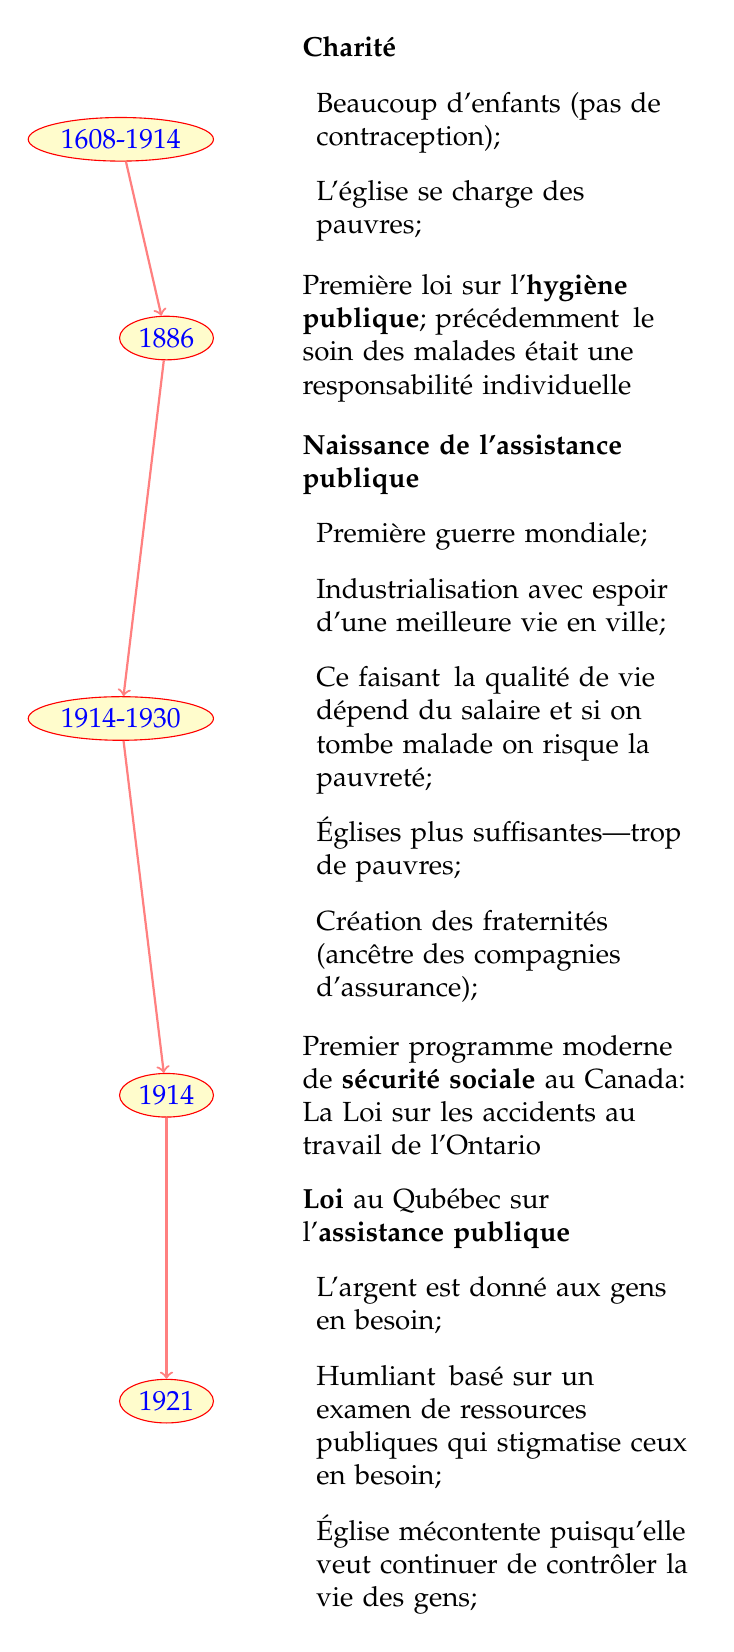
\begin{tikzpicture}[yscale = 0.5,%
           year/.style = {draw	= red,%
           				 text 	= blue,%
           				 fill 	= yellow!20,%
           				 shape 	= ellipse,%
           				 inner sep = 2pt%
           				 },%
           description/.style = {rectangle,%
           				 		align		= left,%
           				 		text width	= 50mm,%
           				 		anchor		= west%
           				 		},%
           timeline/.style = {->,%
           				 	 thick,%
           				 	 red!50%
           				 	 }%
           			]
    \foreach \year/\desc [count=\y] in {%
       1608-1914	/ \textbf{Charité}
       	\begin{itemize}[leftmargin = *]
      		\item	Beaucoup d'enfants (pas de contraception);
      		\item	L'église se charge des pauvres;
      	\end{itemize},%
      	1886	/	Première loi sur l'\textbf{hygiène publique}; précédemment\, le soin des malades était une responsabilité individuelle,%
       1914-1930	/	\textbf{Naissance de l'assistance publique}
       	\begin{itemize}[leftmargin = *]
	       	\item	Première guerre mondiale;
	       	\item	Industrialisation avec espoir d'une meilleure vie en ville;
	       	\item[]	Ce faisant\, la qualité de vie dépend du salaire et si on tombe malade on risque la pauvreté;
	       	\item	Églises plus suffisantes---trop de pauvres;
	       	\item	Création des fraternités (ancêtre des compagnies d'assurance);
       	\end{itemize},%
       	1914	/	Premier programme moderne de \textbf{sécurité sociale} au Canada: La Loi sur les accidents au travail de l'Ontario,%
       	1921	/	\textbf{Loi} au Qubébec sur l'\textbf{assistance publique} 
       	\begin{itemize}[leftmargin = *]
       		\item	L'argent est donné aux gens en besoin;
      	 	\item	Humliant\, basé sur un examen de ressources publiques qui stigmatise ceux en besoin;
     	  	\item	Église mécontente puisqu'elle veut continuer de contrôler la vie des gens;
       	\end{itemize}%
       } { \ifnum\y=1 \node[description](\y){\desc};
           \else\node[description,below=1ex of \z](\y){\desc};
           \fi
           \node[year](y-\y) [left=of \y] {\year};
           \ifnum\y>1\draw[timeline] (y-\z)-- (y-\y);\fi
           \global\let\z=\y% for drawing from last node
       }
\end{tikzpicture}
\begin{tikzpicture}[yscale = 0.5,%
           year/.style = {draw	= red,%
           				 text 	= blue,%
           				 fill 	= yellow!20,%
           				 shape 	= ellipse,%
           				 inner sep = 2pt%
           				 },%
           description/.style = {rectangle,%
           				 		align		= left,%
           				 		text width	= 50mm,%
           				 		anchor		= west%
           				 		},%
           timeline/.style = {->,%
           				 	 thick,%
           				 	 red!50%
           				 	 }%
           			]
    \foreach \year/\desc [count=\y] in {%
       1930-1940		/	\textbf{Premières étapes d'une politique sociale}%
       	\begin{itemize}[leftmargin = *]
	       	\item	\textbf{Crise} de 1929---chômage en forte hausse;
	       	\item	Accroissement des interventions gouvernementales --- le gouvernement est encore timide car il doit avoir le soutien de l'Église;
       	\end{itemize},%
       	1927	/	\textbf{Assurance vieillesse} (\textbf{\textcolor{bulgarianrose}{fédéral}}); programme très strict,%
       	1935	/	\textbf{Hôpitaux provinciaux} au lieu de municipaux; cependant\, encore trop cher pour la majorité de la population,
		1940-1960	/\textbf{Prépondérance \textcolor{bulgarianrose}{fédéral}e}: 
		\begin{itemize}[leftmargin = *]
		  \item	Les besoins engendrés par la guerre règle le problème de chômage;
			\item	Dynamisme du gouvernement \textcolor{bulgarianrose}{fédéral};
			\item	L'idée de donner à \textit{tous} un certain niveau de vie\, et non juste ceux en besoin\, pousse de l'assistance sociale à la sécurité sociale;
		\end{itemize},%
			1940	/	 \textbf{assurance chômage} (\textcolor{bulgarianrose}{fédéral}) Premier programme national,%
			1949	/	 \textbf{allocations familiales} (\textcolor{bulgarianrose}{fédérales}),%
			1952	/	 \textbf{pensions} de \textbf{vieillesse} (\textcolor{bulgarianrose}{fédérales}) non liée à la démonstration du manque de ressources%
       } { \ifnum\y=1 \node[description](\y){\desc};
           \else\node[description,below=1ex of \z](\y){\desc};
           \fi
           \node[year](y-\y) [left=of \y] {\year};
           \ifnum\y>1\draw[timeline] (y-\z)-- (y-\y);\fi
           \global\let\z=\y% for drawing from last node
       }
\end{tikzpicture}

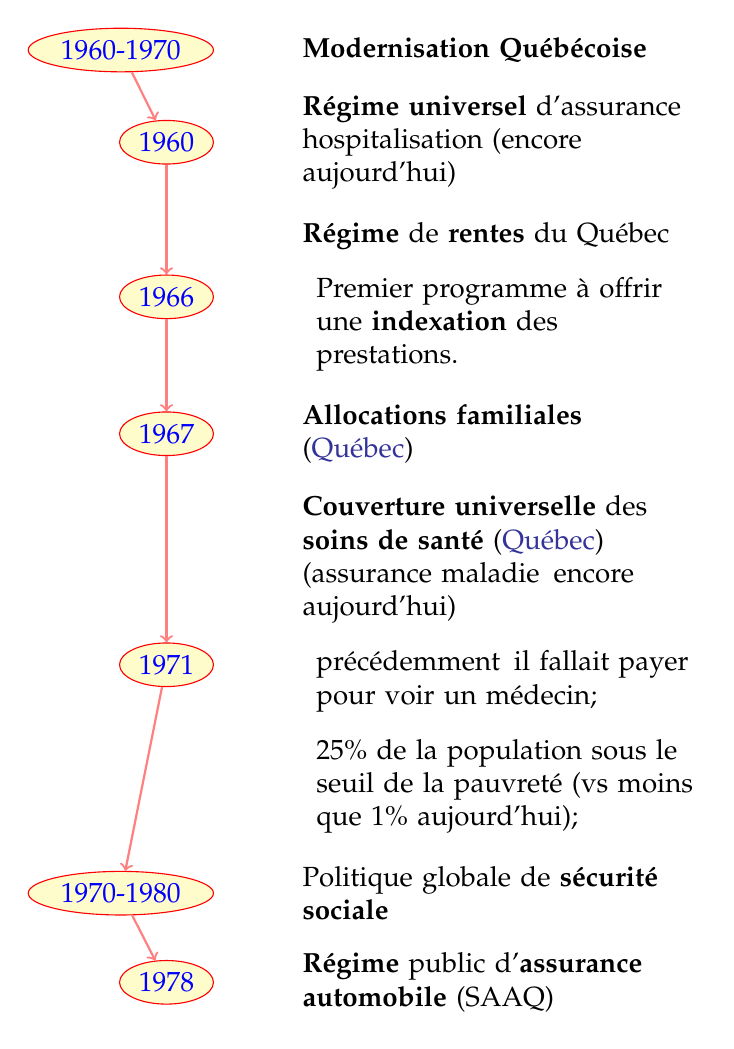
\begin{tikzpicture}[yscale = 0.5,%
           year/.style = {draw	= red,%
           				 text 	= blue,%
           				 fill 	= yellow!20,%
           				 shape 	= ellipse,%
           				 inner sep = 2pt%
           				 },%
           description/.style = {rectangle,%
           				 		align		= left,%
           				 		text width	= 50mm,%
           				 		anchor		= west%
           				 		},%
           timeline/.style = {->,%
           				 	 thick,%
           				 	 red!50%
           				 	 }%
           			]
    \foreach \year/\desc [count=\y] in {%
       	1960-1970	/	\textbf{Modernisation Québécoise},%
			1960		/	\textbf{Régime universel} d'assurance hospitalisation (encore aujourd'hui),%
			1966		/	\textbf{Régime} de \textbf{rentes} du Québec
				\begin{itemize}[leftmargin = *]
				\item	Premier programme à offrir une \textbf{indexation} des prestations.
				\end{itemize},%
			1967	/	 \textbf{Allocations familiales} (\textcolor{blue(pigment)}{Québec}),%
			1971	/	 \textbf{Couverture} \textbf{universelle} des \textbf{soins de santé} (\textcolor{blue(pigment)}{Québec}) (assurance maladie\, encore aujourd'hui)
				\begin{itemize}[leftmargin = *]
				\item	précédemment\, il fallait payer pour voir un médecin;
				\item	25\% de la population sous le seuil de la pauvreté (vs moins que 1\% aujourd'hui);
				\end{itemize},%
       	1970-1980	/	Politique globale de \textbf{sécurité sociale},%
			1978	/	\textbf{Régime} public d'\textbf{assurance automobile} (SAAQ)%
       } { \ifnum\y=1 \node[description](\y){\desc};
           \else\node[description,below=1ex of \z](\y){\desc};
           \fi
           \node[year](y-\y) [left=of \y] {\year};
           \ifnum\y>1\draw[timeline] (y-\z)-- (y-\y);\fi
           \global\let\z=\y% for drawing from last node
       }
\end{tikzpicture}

\textbf{Suite : Recul de la protection Sociale}
\begin{itemize}
	\item	Poussée inflationniste, récession \textbf{(1981-1983)}, taux de chômage élevé;
	\item	Hausse des déficits et baisse des revenus fiscaux, crise de l'endettement public;
	\item	Recul de la protection sociale avec des programmes jugés extravagants;
	\item	Politiques de restriction budgétaire;
	\item	Explosion des coûts de l'assurance maladie
		\begin{itemize}
		\item[1984: ]	Loi canadienne sur la santé---pour préserver l'universalité des soins de santé;
		\end{itemize}
	\item	Coûts d'aucun \og bon sens \fg{} avec un régime qui \textbf{va} devoir changer;
		\begin{itemize}
		\item[1997:]	Assurance médicaments (\textcolor{blue(pigment)}{Québec});
		\item[2006:]	Création d'assurance parentale (\textcolor{blue(pigment)}{Québec});
		\end{itemize}
\end{itemize}

%%%%%%

\begin{conceptgen}{Programmes sociaux au Québec / Canada}
Les 9 fonctions de l'OIT sont couvert par ces programmes:
\begin{itemize}
	\item	Assurance sociale;
	\item	Assurance emploi;
	\item	Allocations familiales;
	\item	Indemnisation accidents travail (CEESST);
	\item	Régime de Rentes du Québec (RRQ);
	\item	Régime de Pension du Canada (RPC);
	\item	Pension sécurité vieillesse (\textcolor{bulgarianrose}{fédéral}) \textbf{\textit{ET}}\\ supplément de revenu garanti (\textcolor{bulgarianrose}{fédéral})\textbf{\textit{ET}}\\ allocation au conjoint ;
	\item	Régime de santé (maladie \textbf{\textit{ET}} hospitalisation---conjoint Canada-Québec);
	\item	\textcolor{amaranth}{Assurance Automobile (\textcolor{blue(pigment)}{Québec}) (SAAQ) (Couvert dans le cours \textit{Introduction à l'actuariat I})} ;
	\item	Assurance parentale (\textcolor{blue(pigment)}{Québec});
	\item	Assurance médicaments (\textcolor{blue(pigment)}{Québec})
\end{itemize}
\end{conceptgen}

Catégories de programmes

\begin{tabularx}{\columnwidth}{| >{\columncolor{airforceblue!80}}>{\setlength\hsize{.25cm}} l | >{\columncolor{beaublue}}X  | >{\columncolor{beaublue}}X	|  >{\columncolor{beaublue}}X  |}
\hline\rowcolor{airforceblue} 
\textcolor{white}{\textbf{Programme}}	&	\textcolor{white}{\textbf{Assistance sociale}}	&	\textcolor{white}{\textbf{Assurance sociale}}		&	\textcolor{white}{\textbf{Régimes universels}}	\\\specialrule{0.1em}{0em}{0em} 
Objectif	&	protection minimale (dernier recourt)	&	protection de base			\\\hline
\end{tabularx}

\textbf{Assistance sociale}

\begin{itemize}[leftmargin = *]
	\item	\textbf{Caractéristiques}:
	\item[]	Test de résidence;
	\item[]	Test de besoin;
	\item[]	Financement gouvernementale (\textcolor{darkgreen}{pay-as-you-go});
	\item	\textbf{Aide Sociale} au \textcolor{blue(pigment)}{Québec}:
	  \item[] Prestations non-imposable;
	  \item[] 3 programmes pour ceux dans le besoin :
		  \begin{enumerate}
		  \item	Programme d'\textbf{assistance sociale} (qui s'appelait le bien-être social);
		  \item	Prime au travail;
			  \begin{itemize}
			  \item	crédit d'impôt qui vise à encourager les individus à faible revenu à rester sur le marché du travail en bonifiant leur offrant un certain soutien financier;
			  \end{itemize}
			 \item	\textbf{Supplément de revenu garanti} (\textit{SRG}) et \textbf{allocation au conjoint} (\textcolor{bulgarianrose}{fédéral});
		  \end{enumerate}
\end{itemize}


\textbf{Assurance sociale}
\begin{itemize}[leftmargin = *]
	\item	\textbf{Caractéristiques}:
	  \item[]	Contributions obligatoires;
	  \item[]	Les prestations sont en fonction de la participation (reliés aux gains);
	  \item[]	Supervision gouvernementale;
	  \item[]	Capitalisation : totale ou partielle;
		  \begin{itemize}
		  \item	L'idée de la capitalisation est que c'est de l'argent mis de côté et pas inclus dans les revenus puisqu'elle sera éventuellement dépensée comme revenu.
		  \end{itemize}
	\item Similitudes avec l'assurance privée:
	  \begin{itemize}
		  \item	Mise en commun des risques
		  \item Description des prestations
		  \item Calcul mathématique des prestations
		  \item Contributions pour financer le coût
		  \item Pas de test de besoins
		  \item Contribue à la sécurité économique
		\end{itemize}
%%%	-----
%%%	NOTES (AJVR):
%%%	+	Développer sur contributions? 
%%%	+	Donner des exemples de programmes obligatoires;
%%%	+	Les prestations ça m'est un peu flou live j'ai moyen compris la façon qu'elle l'a dit mais j'en n'ai pas saise une assez bonne compréhension pour bien l'expliquer, toi?
%%% + va falloir aller lui demander ! Je me fais une liste de questions 
%%%	-----
\begin{center}
\begin{tabular}{| >{\columncolor{beaublue}}c | >{\columncolor{beaublue}}c  |}
\hline\rowcolor{airforceblue} 
\textcolor{white}{\textbf{Avantages}}	&	\textcolor{white}{\textbf{Désavantages}}		\\\specialrule{0.1em}{0em}{0em} 
Protection de base	&	non-universel	\\\hline
Redistribution de l'argent	&	insuffisant	\\\hline
\end{tabular}
\end{center}
%%%	-----
%%%	Comment trouves-tu ce format pour les commentaires? Je trouve ça pourrait être idéal!
%%%	NOTES (AJVR):
%%%	+	Reste à développer sur ceci, voudrait peut-être la peine de ne pas le mettre en forme de tableau mais je me pratiquais;
%%%	+	Ajouter similitude avec assurance privée?
%%% + J'aime ca ! Je vois pas quoi ajouter d'Autres et meme le tableau est clean je trouves ca ok. 
%%%	-----
\end{itemize}
%%%	-----
%%%	Breakdown de tableaux (AJVR):
%%%	Les tableaux c'est compliqué en LaTeX, je t'explique divers composantes ici:
%%%	+	Le premier argument après "begin{tabular}" est l'alignement des colonnes;
%%%	+	"c" pour center, "l" pour left-aligned, "r" pour right-aligned;
%%%	+	les barres "|" ajoute une barre verticale entre colonnes;
%%%	+	on met autant de lettre d'alignement que de colonnes désirées;
%%%	+	"tabular" est l'environnement pour créer les tables;
%%%	+	"airforceblue" est une des couleurs que j'ai défini dans le préambule, airforceblue!80 implique que j'y donne une opacité de 80%;
%%%	+	\columncolor va ensuite appliquer cette couleur à la _colonne_ en entier;
%%%	+	il est entouré de >{} pour y dire d'appliquer cette couleur à la position d'alignement "c"
%%%	+	en revanche, \rowcolor applique une couleur à une _rangée_ en entière;
%%%	+	\hline crée une _ligne_ _h_orizontale;
%%%	+	On sépare les items de la table avec "&" et fini la ligne avec "\\";
%%%	+	\shortstack crée comme une "boite" de texte ce qui fait que je peux créer plusieurs lignes;
%%%	+	Ceci sert uniquement à avoir plusieurs lignes de texte dans une même cellule;
%%%	+	\shortstack[l] est pour y indiquer d'aligner le texte à la gauche.
%%%	-----
\begin{center}
	\textbf{Comparaison d'assurance sociale et privée}
\begin{tabular}{| >{\columncolor{airforceblue!80}}l | >{\columncolor{beaublue}}l  | >{\columncolor{beaublue}}l |}
\hline\rowcolor{airforceblue} 
\textcolor{white}{\textbf{Assurance}}		&	\textcolor{white}{\textbf{Sociale}}		&	\textcolor{white}{\textbf{Privée}}		\\\specialrule{0.1em}{0em}{0em} 
Participation	&	obligatoire	&	facultative		\\\hline
Équité			&	sociale		&	individuelle		\\\hline
Base				&	légale		&	contractuelle	\\\hline
Contexte			&	monopole		&	compétition		\\\hline
\shortstack[l]{Facilité de \\ prévision des\\ coûts}	&	difficile 	&	\shortstack[l]{facile (tout\\ le monde\\ est couvert)}		\\\hline
Capitalisation	&	pas toujours	&	pleinement		\\\hline
\shortstack[l]{Sélection\\ des risques}	&	\shortstack[l]{aucune (peut pas \\ décider d'exclure\\ une personne)}	&	\\\hline
Indexation	&	au coût de la vie	&	rarement		\\\hline
But		&	sécurité sociale	&	\shortstack{couvrir ceux\\ qui le désirent}	\\\hline
\end{tabular}
\end{center}
Donc il y a des similitudes mais leur objectif diffère de façon significative.





\textbf{Régimes universels}
\begin{itemize}[leftmargin = *]
	\item	\textbf{Caractéristiques}:
	  \item[]	Obligatoire et universel;
	  \item[]	Pas de tests de besoins;
	  \item[]	Éligibilité basée sur la résidence (Citoyenneté);
	  \item[]	Prestations fixes définies par la loi;
	  \item[]	Pas de Capitalisation (financés par les recette du gouvernement);
%%%	-----
%%%	NOTES: (AJVR)
%%%	+	J'étais tanné et je n'ai vraiment pas mis beaucoup de détails rendu ici;
%%%	+	Ajouter
%%%	-----
\begin{center}
\begin{tabular}{| >{\columncolor{beaublue}}c | >{\columncolor{beaublue}}c  |}
\hline\rowcolor{airforceblue} 
\textcolor{white}{\textbf{Avantages}}	&	\textcolor{white}{\textbf{Désavantages}}		\\\specialrule{0.1em}{0em}{0em} 
Simple	&	Pas relié aux besoins	\\\hline
Combat la pauvreté	&	Coût caché	\\\hline
	&	Faibles prestations	\\\hline
\end{tabular}
\end{center}
\end{itemize}

Classement des régimes existants

%%%	-----
%%%	NOTES (AJVR):
%%%	+	Ce tableau est à retravailler dans un autre format je crois afin d'ajouter plus de détails d'Isabelle si t'en as, sinon c'est chill je vais faire du reformatting;
%%%	-----
\begin{tabular}{| >{\columncolor{beaublue}}m{3cm} | >{\columncolor{beaublue}}m{3cm} | >{\columncolor{beaublue}}m{3cm} |}
\hline\hline\rowcolor{airforceblue} 
\textcolor{white}{\textbf{Assurance emploi}}						&	\textcolor{white}{\textbf{Assistance sociale}}	&	\textcolor{white}{\textbf{Régimes universels}}	\\\hline
Assurance parentale					&	Assistance sociale						&	Allocations familiales	\\
\hline
Régime de rentes du Québec (R.R.Q.)	&	Prime au travail				&	soins de santé	\\
\hline
Santé Sécurité	au Travail (SST)		&	Supplément de revenu garanti	&	Sécurité de la vieillesse	\\
\hline
Assurance automobile					&	Allocation au conjoint					&	\\
\hline
Assurance médicament					&											&	\\\hline
\end{tabular}

\textbf{Régimes sociaux sous tension}
\begin{itemize}[leftmargin = *]
	\item	Vieillissement de la population;
	\item Changements démographiques (Les \textit{Boomers} sont beaucoup !);
	\item Complexité administrative
	\item Évolution de la société depuis leur mise en place;
	  \begin{itemize}
	  \item Par exemple, la \textit{rente du Survivant}. Le salaire ne vient plus seulement du mari, à revoir ? 
	  \end{itemize}
	\item Répartition de la richesse
	\item Abus
	\item La mondialisation mène à la compétition
	  \begin{itemize}
	  \item Maintenant qu'on sait ce que les autres pays font, on sait ce qui se fait mieux, on veut compétitionner
	  \end{itemize}
\end{itemize}
Nos régimes craquent d'un peu partout. On mets en vigueur des changements et des lois pour cacher ces fissures, mais ça va sans doute exploser un jour.

\textbf{Les États-Unis}

\begin{itemize}[leftmargin = *]
	\item	Les droits sociaux ne sont pas dans la constitution;
	\item Vision différente:
	  \begin{itemize}
	  \item Selon eux, la meilleure assistance sociale reste le plein emploi : ils cherchent à maintenir la croissance économique et à faire baissser le chômage.
	  \end{itemize}
	\item Protection des démunis : axée sur l'aide sociale plutôt que la sécurité;
	  \begin{itemize}
	  \item On s'occupe des pauvres après (mesure humiliante : \textit{food ticket} pour l'épicerie)
	  \item 6 volets à la sécurité sociale:
	  \begin{enumerate}
	    \item Vieillesse et décès (survivants) (\textcolor{bulgarianrose}{fédéral})
	    \item Invalidité (\textcolor{bulgarianrose}{fédéral})
	    \item Médicare (Medicaid) (\textcolor{bulgarianrose}{fédéral})
	    \item Chômages (États)
	    \item Accidents de travail et maladies professionnelles (États)
	    \item Assurance maladie (Obama Care)
	  \end{enumerate}
	\item Obama Care (détails) : 
	  \begin{itemize}
	    \item Obligation aux individus de souscrire si non-couvert par leur employeur
	    \item Interdiction de refuser de couvrir un individu en raison d'antécédents médicaux (du côté des assureurs)
	    \item le gouvernement accorde de l'aide pour payer la prime si le revenu est entre 1 à 4 fois le seuil de la pauvreté
	    \item \textbf{supprimé le 1er Janvier 2019 }
	    \item Certains états ont maintenu l'obligation de détenir de l'assurance maladie
	    \item[] Exemple : \textit{Massachussett}, \textit{New Jersey} et \textit{Columbia}
	 \end{itemize}
	 \end{itemize}
	 \end{itemize}
 Les raisons d'un tel régime était qu'au \textit{États-Unis}, 64\% des faillites étaient liées aux frais de santé
\newpage

\section{Le système de retraite au Canada}

\begin{definitionNOHFILL}[Vie active]
Période de vie où 
\begin{itemize}[leftmargin = *]
	\item	On est \textbf{actif} sur le \textbf{marché du travail};
	\item	Les \textbf{revenus} proviennent principalement de revenus \textbf{d'emploi}.
\end{itemize}
\end{definitionNOHFILL}

\begin{definitionNOHFILL}[La retraite]
Période de la vie où l'on est, ou considéré comme étant, \textbf{incapable de travailler}. Il s'ensuit que le revenus ne provient pas d'emploi.

\begin{conceptgen}{Objectifs de la protection}
\begin{itemize}[leftmargin = *]
	\item	Compenser la \textbf{perte de revenu} associée à la retraite;
	\item	Contrer la pauvreté des personnes âgées;
	\item	Maintenir en emploi ou favoriser le retrait des travailleurs âgés (Incitatif).
\end{itemize}
\end{conceptgen} 

\begin{conceptgen}{\textbf{Types de revenus} à la retraite}
\begin{itemize}[leftmargin = *]
	\item	Rentes de l'état: gouvernement paye des rentes (régime public, souvent insuffisant);
	\item[] RRQ, PSV;
	\item	Rentes de l'employeur: certains employeurs payent des rentes (régime privé);
	\item	Épargne personnelle (patrimoine): la proportion du revenu dépend de l'épargne de l'individu;
	\item	Aide sociale pour personnes âgées;
	\item[] SRG pour les plus démunis.
\end{itemize}
\end{conceptgen} 
\end{definitionNOHFILL}

%%%

\begin{definitionNOHFILL}[Âge normal de retraite (ANR)]
Âge de début de retraite utilisée pour le calcul des prestations payables à la retraite. Cet âge est loin de l'âge effectif de la retraite actuel, il s'agit simplement de l'âge théorique utilisé pour les calculs.

\begin{rappel_enhanced}[Historique]
\begin{itemize}[leftmargin = *]
	\item	L'ANR est de 65 ans depuis 1970 (Harper avait décidé d'augmenter cet âge graduellement entre 2023 et 2029, Trudeau est venu contre cette décision);
	\item	Dans le passé, l'ANR était de 65 ans pour les hommes et 60 ans pour les femmes---cette pratique maintenant considérée discriminatoire et interdite;
	\item	Les régimes publics l'utilisent et c'est l'âge maximal permis pour les régimes privés;
	\item	Ce n'est pas un âge obligatoire pour les contribuables.
\end{itemize}
\end{rappel_enhanced}

\begin{conceptgen}{Retraite anticipée}
\begin{itemize}[leftmargin = *]
	\item	Prendre sa retraite plus tôt implique une \textbf{réduction actuarielle};
	\item	La loi peut prévoir qu'une rente sans réduction peut être versée à \textit{certaines conditions};
		\begin{itemize}[leftmargin = *]
		\item	Par exemple, selon le \textbf{nombre d'années de service}, comme dans l'armée, une pension complète peut-être payée après seulement 25 ans.
		\end{itemize}
	\item	\textcolor{red}{Ce sujet est vu plus en profondeur dans les cours de Régimes de retraites.}
\end{itemize}
\end{conceptgen} 
\end{definitionNOHFILL}

\begin{rappel_enhanced}[Historique de la retraite]
Historiquement, la retraite était rare et courte. Avec l'augmentation de l'espérance de vie est venu des changements majeurs au niveaux de la durée de la retraite. 

Ce tableau illustre assez bien l'historique de la retraite:

\centerline{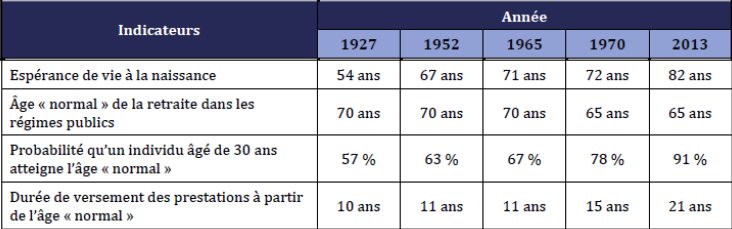
\includegraphics[scale=0.32]{src/ACT-1005/retraite-age-hist.png}}

\begin{itemize}[leftmargin = *]
		\item	La vie active a donc diminué avec la \textbf{diminution de l'ANR} et la \textbf{retraite anticipé};
		\item	La durée de la retraite est passée de 10 à 21 ans, menant à de grandes \textbf{pressions financières} sur le système de retraite;
		\item	De plus, le coût de la vie a augmenté et cette \textbf{inflation} \textit{multiplie les pressions} sur les \textbf{longues périodes de paiements} (20 ans et plus).
\end{itemize}
\end{rappel_enhanced}

%%%

\begin{rappel_enhanced}[Baby Boom]
\begin{itemize}[leftmargin = *]
	\item	Génération d'enfants nés après la fin de la Deuxième Guerre mondiale (taux de natalité élevé);
	\item[]	Nés dans les alentours \textit{approximatifs} de 1946 à 1965.
	\item	Le nombre moyen d'enfants par femme était de 3.7 (4.1 dans les années 50);
	\item[]	En contraste, c'est de 1.6 enfants par femme aujourd'hui.
	\item	Le départ des baby-boomers à la retraite a un impact socio-économique important.
	\item[] principalement car les hauts taux de natalité ne seront pas renouvelés.
\end{itemize}
\end{rappel_enhanced}

\begin{rappel_enhanced}[Baby Bust (génération X)]
\begin{itemize}[leftmargin = *]
	\item	Enfants nés dans les alentours \textit{approximatifs} de 1966 à 1976.
	\item	Génération coincée entre les baby-boomers et la génération Y;
	\item	Difficulté à trouver des emplois en raison du grand nombre de baby-boomers.
\end{itemize}
\end{rappel_enhanced}

\begin{conceptgen}{Proportion de la population active}
Les graphiques de pyramides d'âges permettent la visualisation de l'augmentation importante de la population âgée. L'\textbf{insuffisance} de la \textbf{population active} pour \textbf{soutenir} le \textbf{régime de retraite} actuel s'ensuit.

En \textbf{contraste} aux \textbf{États-Unis} (1.9\%) et le \textbf{reste du Canada} (5.1\%), la \textbf{population active du \textcolor{blue(pigment)}{Québec}} entre 20 et 64 ans va \textbf{diminuer} (-3.6\%) de 2015 à 2030. 
\end{conceptgen} 

\begin{itemize}[leftmargin = *]
	\item	Enfants nés dans les alentours \textit{approximatifs} de 1966 à 1976.
	\item	Génération coincée entre les baby-boomers et la génération Y;
	\item	Difficulté à trouver des emplois en raison du grand nombre de baby-boomers.
\end{itemize}
%%%

\begin{conceptgen}{Approches des régimes de retraite}
\textbf{Beveridge}
\begin{itemize}[leftmargin = *]
	\item	Approche d'une rente \textbf{universelle};
	\item	Verse à tous les individus une rente;
	\item	Prestations aux démunis.
\end{itemize}
\tcbline
\textbf{Bismark}
\begin{itemize}[leftmargin = *]
	\item	Approche d'une rente pour les \textbf{travailleurs}.
\end{itemize}
\end{conceptgen}

\begin{conceptgen}{Adhésion à un régime de revenu à la retraite}
Les régimes peuvent être \textbf{obligatoires} ou \textbf{volontaires}.

\textbf{Obligatoire}
\begin{itemize}[leftmargin = *]
	\item	Tous les individus doivent cotiser pour leurs retraites;
	\item	Garanti que tout le monde se constitue une retraite.
\end{itemize}

\textbf{Volontaire}
\begin{itemize}[leftmargin = *]
	\item	Les gens ont tendance à sous-estimer leurs besoins futurs et ne pas épargner suffisamment d'argent;
	\item	La présence d'un système obligatoire n'empêche pas celle d'une épargne supplémentaire par un régime facultatif;
\end{itemize}

\begin{center}
	\textbf{Exemples}
\end{center}

\textbf{État}
\begin{itemize}[leftmargin = *]
	\item	Pension de la sécurité de vieillesse (PSV) \textcolor{brickred}{(obligatoire)};
	\item	Régie des rentes du Québec (RRQ) \textcolor{brickred}{(obligatoire)}.
	\item	Régime de Pension du Canada (RPC) \textcolor{brickred}{(obligatoire)}.
\end{itemize}
\textbf{Privé}
\begin{itemize}[leftmargin = *]
	\item	Régimes complémentaires de retraite (RCR) \textcolor{brickred}{(habituellement obligatoire s'il est présent)};
	\item	Régime \textbf{volontaire} d'épargne-retraite (RVER) \textcolor{blue}{(facultatif)};
	\item	Régime enregistré d'épargne-retraite (REER) \textit{collectif} \textcolor{blue}{(facultatif)}.
\end{itemize}
\textbf{Individuel} \textcolor{blue}{(facultatifs)}
\begin{itemize}[leftmargin = *]
	\item	Compte d'épargne libre d'impôt (CELI), REER, épargne, biens (maisons, \dots).
\end{itemize}
\end{conceptgen}

\begin{conceptgen}{Financement}
\begin{center}
\textbf{Capitalisation} (\textbf{funded})
\end{center}

\textbf{Procédure}
\begin{enumerate}[leftmargin = *]
	\item	Participants actifs versent leurs cotisations;
	\item	Le régime place les sommes au nom de chaque participant;
	\item	Au moment de la retraite, ces mêmes montants lui sont restitués sous forme de rente.
\end{enumerate}

\textbf{Détails}
\begin{itemize}[leftmargin = *]
	\item	Il est possible d'avoir une capitalisation totale ou partielle;
	\item	Les sommes sont considérables et servent de financement pour les gouvernements et industries;
	\item	Fonctionnement se rapproche à celui d'une compagnie d'assurance.
\end{itemize}

\textbf{Risques}
\begin{itemize}[leftmargin = *]
	\item	\textbf{Fluctuations} de l'économie;
	\item	\textbf{Faillites} d'entreprises;
	\item	\textbf{Corruption} (malversations).
\end{itemize}

\tcbline

\begin{center}
\textbf{Répartition} (\textcolor{darkgreen}{Pay-as-you-go (PAYG)})
\end{center}

\textbf{Procédure}:
\begin{enumerate}[leftmargin = *]
	\item	Participants actifs versent leurs cotisations;
	\item	Le régime utilise les sommes pour payer les pensions des retraités actuels.
\end{enumerate}

\textbf{Détails}
\begin{itemize}[leftmargin = *]
	\item	Repose sur une forte solidarité entre générations;
	\item	Sa viabilité dépend du rapport entre le nombre de cotisants et le nombre de personnes retraitées;
	\item	Aucun actif mis de côté;
	\item	Dois presque forcément être un régime obligatoire et public.
\end{itemize}

\textbf{Risques}
\begin{itemize}[leftmargin = *]
	\item	Dépend de la \textbf{croissance de la masse salariale} puisque les cotisations sont prélevés sur les payes;
\end{itemize}
\end{conceptgen}

\begin{conceptgen}{Paliers du système équilibré canadien de la retraite}
\centerline{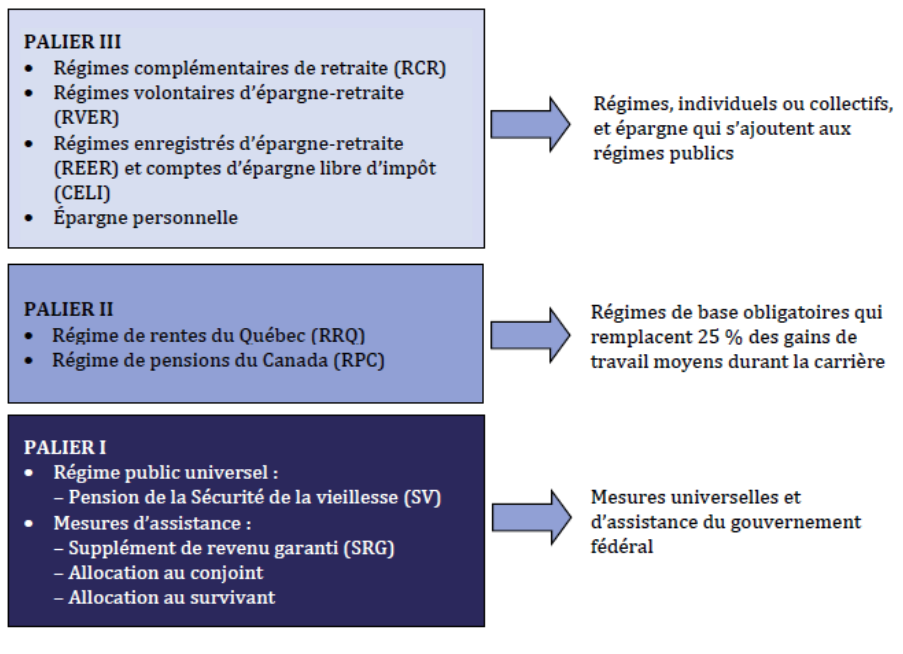
\includegraphics[scale=0.25]{src/ACT-1005/retraite-paliers.png}}

\textbf{Palier I et II}
\begin{enumerate}[leftmargin = *]
	\item	Composante \textbf{publique};
	\item	But d'\textbf{éliminer} au maximum la \textbf{pauvreté} des personnes âgées;
	\item	\textbf{Répartit les revenus} des gens tout au long de leur vie pour assurer un certain niveau de remplacement de revenu.
\end{enumerate}

\textbf{Palier III}
\begin{enumerate}[leftmargin = *]
	\item	Composante \textbf{privée}.
\end{enumerate}
\end{conceptgen}

\begin{conceptgen}{Remplacement de revenu à la retraite}
\paragraph{Principe de base}Règle générale qu'on doit compter sur un remplacement de 70\% de son revenu avant la retraite afin de maintenir le \textbf{même} niveau de vie. Cela ne tient pas compte cependant du \textbf{niveau de revenu} ni du \textbf{type de retraite} visé.
\\

Raisons pourquoi pas 100\%:
\begin{itemize}[leftmargin = *]
	\item	Dépenses transport moindre;
	\item	Fin de dépenses hypothécaires;
	\item	Départ d'enfants (études, nourriture, \dots);
	\item	Dépenses générales moindres (rabais, \dots);
	\item	Fin des charges sociales (parents à charge);
	\item	Fin de l'épargne retraite.
\end{itemize}
\tcbline
\textbf{Provenance} de revenu à la retraite
\begin{itemize}[leftmargin = *]
	\item	L'objectif des régimes gouvernementaux est de remplacer $Y\%$ pour les personnes gagnant un certain salaire;
	\item	Ce salaire, appelé le \textbf{maximum des gains admissibles} (\textit{MGA}), est déterminé annuellement par la \textit{RRQ};
	\item	L'importance de chaque palier va donc varier entre individus selon leur revenu.
	\item[] Plus les revenus de travail moyens sont faibles avant le retrait du marché du travail, plus les régimes publics jouent un rôle important (les gens à faibles revenus n'aurons pas assez d'argent pour en mettre de côté) 
\end{itemize}
\end{conceptgen}

\newpage

\section{Loi sur la sécurité de la vieillesse}

\begin{conceptgen}{Types de prestations}
Il existe plusieurs types de prestations dont:
\begin{itemize}[leftmargin =  *]
	\item	\hyperref[sec:PSV]{Pension de la sécurité de la vieillesse (\textit{PSV})};
	\item	\hyperref[sec:SRG]{Supplément du revenu garantie (\textit{SRG})};
	\item	\hyperref[sec:Alloc]{Allocation (au conjoint)};
	\item	\hyperref[sec:Alloc_survival]{Allocation (de survivant)}.
\end{itemize}
\end{conceptgen}

\begin{rappel_enhanced}[Historique]
%%%	--------------
%%%	NOTE
%%%	+	Voir cette page de "l'encyclopédie canadienne" (https://www.thecanadianencyclopedia.ca/fr/article/pension-de-vieillesse);
%%% +   Intéressant, explique bien en détail avec une meilleure idée sur les contextes de l'époque. (OC)
%%%	--------------
\begin{description}
	\item[1952]	Entrée en vigueur de la loi de la sécurité et vieillesse;
		\begin{itemize}[leftmargin = *]
		\item	Programme \textcolor{bulgarianrose}{fédéral};
		\item	Au niveau \textcolor{blue(pigment)}{provincial}, il n'y a pas encore grand-chose de développé;
		\item	Idée de \hl{garantir à \textbf{tous}} les citoyens \hl{âgés} (70 ans et plus) une \hl{pension non-liée au revenu} avec la PSV.
		\end{itemize}
	\item[1966]	Entrée en vigueur du \textit{RCP} et \textit{RRQ};
		\begin{itemize}[leftmargin = *]
		\item	Inclut une révision de la \textit{PSV}---élargir la portée, revoir le programme, etc.;
		\item	Programmes obligatoires.	
		\end{itemize}
	\item[1967]	Entrée en vigueur du \textit{SRG}
		\begin{itemize}[leftmargin = *]
		\item	Supplément au \textit{PSV} temporaire jusqu'au début des paiements du \textit{RCP} et \textit{RRQ};
		\item	Initialement supposé être temporaire pour aider ceux déjà à la retraite, car le \textit{RCP} et \textit{RRQ} n'allaient pas payer de prestations avant 10 ans;
		\item	Diminution de l'âge d'admissibilité à 65 ans;
		\item	Augmentation du montant des pensions.
		\end{itemize}
%%%	--------------
%%%	NOTE
%%%	+	Je trouves ça hyper pertinent, mais penses-tu qu'on devrait se limiter au contenu du cours ? (je penses à ceux qui paniquent pour rien en lisant du "nouveau contenu")(OC)
%%%	+	Ajout de colour code --- orange pour l'extra (AJVR)
%%%	--------------
	\item[1975]	Entrée en vigueur de l'Allocation au conjoint ;
		\begin{itemize}[leftmargin = *]
		\item	{\color{burntorange} Lorsqu'un seul membre du couple reçoit la \textit{PSV} et le \textit{RSG} et que l'autre a entre 60 et 64 ans;
		\item	Éventuellement renommé \og Allocation \fg{}.}
		\end{itemize}
	\item[1985]	Entrée en vigueur de l'allocation au conjoint veuf.
		\begin{itemize}[leftmargin = *]
		\item	{\color{burntorange} Extension à l'allocation au conjoint pour inclure les veuf(ve)s à faible revenu entre 60 et 64 ans dont le conjoint décédé était prestataire de la PSV et le RSG;
		\item	Éventuellement renommé \og allocation de survivant \fg{}.}
		\end{itemize}
\end{description}
\end{rappel_enhanced}

\subsection{Pension de sécurité à la vieillesse (\textit{PSV})}
\label{sec:PSV}
\begin{definitionNOHFILL}[Définition]
Régime \textbf{universel} assurant un revenu \textit{minimum} à la retraite tout citoyen canadien \textbf{admissible}. 
\hl{Le but est de couvrir \textit{environ} 15\% des revenus avant retraite} pour le \hl{travailleur moyen}.
\end{definitionNOHFILL}

\begin{conceptgen}{Admissibilité}
\begin{itemize}[leftmargin = *]
	\item	Sujet à un \hl{test de résidence}---doit: 
		\begin{enumerate}[leftmargin = *]
		\item	être citoyen canadien \\
					\textbf{ou}\\
				être un résident autorisé;
		\item	avoir habité au Canada pendant au moins 10 ans après l'âge de 18 ans;
		\end{enumerate}
	\item	Si quitte le Canada, doit avoir habité au Canada pendant au moins 20 ans après l'âge de 18 ans;
	\item[]	\textbf{Note}: Il y existe d'autres possibilités selon ententes avec d'autres pays (comme les É.-U.);
	\item	Pas de test de besoin, mais possibilité de devoir la rembourser (\hypertarget{recup_tx_l8r1}{\hyperlink{recup_tx_explain}{\textcolor{blue_rectangle}{impôt de récupération}}});
	\item   Aucun critère lié au travail;
	\item	Doit être d'au moins l'ANR (65 ans), mais \textit{pas besoin d'être retraité};
\end{itemize}
\end{conceptgen}

\begin{conceptgen}{Montant de la rente}
Établi selon le nombre d'années où l'individu a habité au Canada après l'âge de 18 ans.

\paragraph*{Pension complète}
\begin{itemize}[leftmargin = *]
	\item	Si 40 ans de résidence au Canada après l'âge de 18 ans;
	\item	Dont au moins 10 ans immédiatement avant la demande \\
				\textbf{ou} 	\\
			1 an de résidence avant la demande et 3 ans de résidence avant l'âge de 55 ans pour chaque année manquante du 10 ans.
\end{itemize}

\paragraph*{Pension partielle}
\begin{itemize}[leftmargin = *]
	\item	Au moins 10 ans de résidence au Canada après l'âge de 18 ans;
	\item	Un quarantième (1/40) de la pension pour chaque année après 18 ans;
	\item	Une pension partielle \textbf{ne} peut \textbf{pas} être augmentée après son approbation en fonction du nombre d'années de résidence supplémentaire.
\end{itemize}
\end{conceptgen}

\begin{conceptgen}{Particularités du paiements}
\begin{description}
	\item[Étranger]	Avoir vécu au Canada pendant au moins 20 ans après l'âge de 18 ans;
		\begin{itemize}[leftmargin = *]
		\item	Note que l'on ne peut pas être absent du Canada pour plus que 6 mois sans perdre son droit de cumuler;
		\item   Le temps avant le départ n'est pas perdu, il est possible de continuer à cumuler à partir du retour du voyage.
		\end{itemize}
	\item[Report] En échange d'une pension plus élevée, il est possible depuis juillet 2013 de reporter la PSV jusqu'à 5 ans;
		\begin{itemize}[leftmargin = *]
		\item	Augmentation de 0.6\% pour chaque mois de report jusqu'à un maximum de 36\% à l'âge de 70 ans (modification actuarielle).
		\item   L'impôt de récupération explique pourquoi certaines personnes pourraient vouloir reporter leur PSV (\textcolor{red}{expliqué plus tard}).
		\end{itemize}
	\item[Indexation]	Le montant de la rente est indexé à l'IPC à chaque trimestre.
\end{description}
\end{conceptgen}

\begin{conceptgen}{Fiscalité}
\begin{itemize}[leftmargin = *]
	\item	La prestation est imposable (\textcolor{bulgarianrose}{fédéral} et \textcolor{blue(pigment)}{provincial});
	\item	Depuis 1989, il existe un \hypertarget{recup_tx_explain}{\hyperlink{recup_tx_l8r1}{\textcolor{blue_rectangle}{impôt de récupération}}} qui s'impose lorsque le revenu excède un certain seuil;
	\item	Le seuil de revenu maximal en 2019 était de 77 580\$ et donc la récupération serait 15\% du revenu net \textbf{en excès de} ce montant (celle-ci n'est donc pas universelle);
	\item	Il est possible de récupérer la PSV en entier (dès 126 058\$);
	\item	Puisque \hl{le test de revenu est individuel} et non par couple, il est possible d'être créatif avec ses finances.
\end{itemize}
\end{conceptgen}

\begin{conceptgen}{Âge à la retraite}
	\begin{itemize}[leftmargin = *]
		\item	Le gouvernement \textit{Harper} avait annoncé en 2012 l'intention de hausser graduellement l'âge de la retraite de 65 à 67 ans (2023-2029);
				\begin{itemize}[leftmargin = *]
				\item Le but était d'assurer la préservation du programme, compte tenu de l'augmentation de l'espérance de vie à la hausse.
				\end{itemize}
		\item	Le gouvernement \textit{Trudeau} a annoncé l'annulation de l'intention de hausser de l'\textit{ANR} en 2016;
		\item	La \hl{raréfaction de la main d'oeuvre} va mettre une \hl{pression} sur les travailleurs de \hl{rester sur le marché du travail plus longtemps};
		\item	L'ICA a pris position publiquement en avril 2019 pour une augmentation de l'ANR en échange de prestations plus élevées.
				\begin{itemize}[leftmargin = *]
				\item Pour la \textit{PSV}, cela impliquerait une prestation payable à 67 ans au lieu de 65 ans.
				\item Un revenu encore plus élevé à la retraite assurerait une meilleure protection contre les coûts associés au risque de longévité.
				\end{itemize}
	\end{itemize}
\end{conceptgen}

\begin{conceptgen}{Financement}
Le financement de la \textit{PSV} est \textcolor{darkgreen}{pay-as-you-go}, il n'y a pas de caisse distincte et sort directement des impôts.
\begin{itemize}[leftmargin = *]
	\item En raison du vieillissement de la population, le coût du programme augmente à un taux très supérieur à la croissance du \textit{PIB}.
\end{itemize}
\end{conceptgen}

\columnbreak

\subsection{Supplément de revenu garanti (\textit{SRG})}
\label{sec:SRG}
\begin{definitionNOHFILL}[Définition]
Prestation mensuelle non imposable offerte aux bénéficiaires de la \textit{PSV} ayant un faible revenu résidant au Canada. 
\end{definitionNOHFILL}

\begin{conceptgen}{Admissibilité}
\begin{itemize}[leftmargin = *]
	\item	Recevoir la \textit{PSV}---le \textit{SRG} peut être reçu en même temps que la \textit{PSV};
	\item	Avoir des gains faibles---prestation réduite selon les autres revenus de la personne ou du conjoint.
\end{itemize}
\end{conceptgen}

\begin{conceptgen}{Montant de la prestation}
Établi en fonction de l'état conjugal et du revenu de l'année précédente.\\

La définition de revenus:
\begin{description}
	\item[exclus]	la \textit{PSV} et l'allocation;
	\item[inclus]	\textit{RRQ}, \textit{REER}, \textit{RCR}, placements, loyers, gains en capitaux, emplois, etc.
\end{description}

\textbf{Montants maximaux} mensuels (\textit{1$^{\text{er}}$ Janvier 2020}):
\begin{itemize}[leftmargin = *]
	\item	Personne seule et personne ayant un conjoint qui ne \textit{reçoit pas la PSV} : 916.38\$;
	\item	Personne ayant un conjoint qui \textit{reçoit la PSV ou l'Allocation} : 551.63\$;
\end{itemize}

\textbf{Caractéristiques} : 
\begin{itemize}[leftmargin = *]
	\item	Depuis 2008, il est possible d'avoir jusqu'à 3 500\$ de revenus d'emploi sans impact sur la prestation---ce montant \textit{devrait} augmenter à 5 000 \$ en 2020 avec une pénalité de seulement 50\% pour les 10 000\$ suivants;
	\item	Réduction de 1\$ pour chaque 2\$ de revenu autre;
	\item	Le montant est déterminé annuellement selon les gains de l'année précédente et donc il peut fluctuer dans le temps.
\end{itemize}
\end{conceptgen}

\begin{conceptgen}{Particularités du paiement}
\begin{description}
	\item[Étranger]	Aucune prestation pour le non-résident du Canada;
	\item[Indexation]	Le montant de la rente est indexé à l'IPC à chaque trimestre;
	\item[Fiscalité]	Aucune imposition des montants de SRG;
	\item[Financement]	Par répartition (\textcolor{darkgreen}{pay-as-you-go});
\end{description}
\end{conceptgen}

\begin{conceptgen}{Cessation des paiements}
\begin{itemize}[leftmargin = *]
	\item	Si l'individu (couple) ne soumet pas de déclaration de revenus;
	\item	Départ pour plus de 6 mois consécutifs;
	\item	Revenu(s) supérieur au montant maximal établit pour l'année;
	\item	Incarcération;
	\item	Décès.
\end{itemize}
\end{conceptgen}

\columnbreak

\subsection{Allocation}
\label{sec:Alloc}
\begin{definitionNOHFILL}[Définition]
Prestation mensuelle payable à une personne entre 60 et 64 ans conjoint d'un prestataire du \textit{SRG} (anciennement appelée Allocation au conjoint, existe depuis 1975).
\end{definitionNOHFILL}

\begin{conceptgen}{Admissibilité}
\begin{itemize}[leftmargin = *]
	\item	Être conjoint d'un prestataire de la \textit{PSV} et du \textit{SRG};
	\item	Être âgé de 60 à 64 ans;
	\item	Citoyen canadien \\
			\textbf{ou}\\
			résident autorisé;
	\item	Habiter au Canada;
	\item	Avoir vécu au Canada pendant au moins 10 ans après l'âge de 18 ans;
	\item	Présenter une nouvelle demande annuellement;
	\item	Avoir des revenus faibles (le revenu combiné du couple, excluant PSV et SRG, ne doit pas excéder un certain seuil).
\end{itemize}
\end{conceptgen}

\begin{conceptgen}{Montant de la prestation}

\begin{itemize}[leftmargin = *]
	\item	Le maximum est la somme du PSV et SRG maximal au taux du couple marié---en 2018 ceci était de 1 141.08\$ par personne;
	\item	Aucune allocation si les autres revenus du couple excèdent 33 696\$;
	\item	Il y a des particularités sur la réduction du paiement.
			\begin{itemize}[leftmargin = *]
			\item   Allocation réduite selon les revenus autres que la \textit{PSV}, \textit{SRG} de 3\$ par 4\$ de revenus jusqu'à ce que le montant soit égal à la \textit{PSV};
			\item   Réduit de 1\$ par 4\$ de revenu ensuite. 
			\end{itemize}
\end{itemize}
\end{conceptgen}

\begin{conceptgen}{Cessation des paiements}
	\begin{itemize}[leftmargin = *]
		\item	Le couple ne soumet pas de déclaration de revenus;
		\item 	Le revenus du couple est supérieur au maximum définit;
		\item 	Le conjoint n'est plus admissibles au \textit{SRG};
		\item 	Départ pendant plus de 6 mois;
		\item 	Divorce ou séparation;
		\item 	Incarcération;
		\item	Atteinte de 65 ans;
		\item	Décès
			\begin{itemize}[leftmargin = *]
			\item	Du conjoint;
			\item 	De la personne qui reçoit l'Allocation.
			\end{itemize}
	\end{itemize}
\end{conceptgen}

\columnbreak

\subsection{Allocation au survivant}
\label{sec:Alloc_survival}
\begin{conceptgen}{Admissibilité}

\begin{definitionNOHFILL}[Définition]
Prestation mensuelle payable à une personne entre 60 et 64 ans veuf(ve) (existe depuis 1985).
\end{definitionNOHFILL}

\begin{itemize}[leftmargin = *]
	\item	Être veuf(ve);
	\item	Être âgé entre 60 et 64 ans;
	\item	Citoyen canadien \\
			\textbf{ou}\\
			résident autorisé;			
	\item	Avoir vécu au Canada pendant au moins 10 ans après l'âge de 18 ans;
	\item	Avoir des revenus faibles.
\end{itemize}
\end{conceptgen}

\begin{conceptgen}{Montant de la prestation}
\begin{itemize}[leftmargin = *]
	\item	Le maximum est de 1 360.20 \$.
	\item	Aucune allocation si les autres revenus excèdent 24 552\$;
	\item	Il y a des particularités sur la réduction du paiement.
		\begin{itemize}[leftmargin = *]
		\item   Allocation réduite selon les revenus autres que la \textit{PSV}, \textit{SRG} de 3\$ par 4\$ de revenus jusqu'à ce que le montant soit égal à la \textit{PSV};
		\item   Réduite de 1\$ par 2\$ de revenu ensuite. 
		\end{itemize}
\end{itemize}
\end{conceptgen}

\begin{conceptgen}{Cessation des paiements}
\begin{itemize}[leftmargin = *]
	\item	Si les revenus de l'individu deviennent suffisants;
	\item 	Départ pendant plus de 6 mois;
	\item	Se remarie (ou union de fait) pendant plus de 12 mois;
	\item 	Atteinte de 65 ans;
	\item	Décès.
\end{itemize}
\end{conceptgen}


%%%
%%% PARLER DE LA SECTION "LE FUTUR... "? (OC)
%%%	Je l'ai exclus puisque je trouvais que ça recoupais et j'ai ajouté d'autres notes dans le reste du chapitre pour la balance (AJvR)
%%%

\newpage

\section{Le régime des rentes du Québec}

\begin{conceptgen}{Raison d'être}
\begin{itemize}[leftmargin = *]
	\item	Régime d'assurance sociale;
	\item	Offrir une \hl{protection financière de base aux travailleurs} (et leurs proches) à la \textit{retraite}, au \textit{décès} ou en cas d'\textit{invalidité};
	\item	Le \textcolor{blue(pigment)}{Québec} est la seule province à avoir son propre régime public de pensions qui couvre tous les emplois au \textcolor{blue(pigment)}{Québec}.
\end{itemize}

\textbf{Caractéristiques}
\begin{description}
	\item[Public]	Administré entièrement par des organismes de l'état;
	\item[Universel]	Mais basé sur le travail (\textit{approche bismarckienne});
	\item[Obligatoire]	Tous les travailleurs sont obligés de cotiser;
	\item[Contributif]	Les cotisations des travailleurs et employeurs supportent les prestations du régime;
	\item[Autofinancé]	Tout comme les prestations, les coûts d'administration proviennent des cotisations;
	\item[Imposable]	Les prestations reçues sont imposables;
	\item[Transférable]	Le régime est pancanadien vers le RPC;
	\item[Indexé]	Le régime est indexé de 2 façons:
		\begin{enumerate}[leftmargin = *]
		\item	Lors du calcul initial des prestations;
		\item	L'augmentation des rentes déjà en paiement.
		\end{enumerate}
\end{description}
\end{conceptgen}

\begin{conceptgen}{Types de prestations}
\begin{description}
	\item[Retraite]	
		\begin{itemize}[leftmargin = *]
		\item	Rente de retraite (RR).
		\end{itemize}
	\item[Invalidité]	
		\begin{itemize}[leftmargin = *]
		\item	Rente d'invalidité (RI);
		\item	Rente d'enfant de personne invalide;
		\item	Montant additionnel pour invalidité pour les bénéficiaires de la RR.
		\end{itemize}
	\item[Décès]	
		\begin{itemize}[leftmargin = *]
		\item	Rente de conjoint survivant (RCS);
		\item	Rente d'orphelin (RO);
		\item	Prestation de décès.
		\end{itemize}
\end{description}
\end{conceptgen}

\begin{rappel_enhanced}[Mise en place]
\begin{description}
	\item[1966]	Entrée en vigueur;
		\begin{itemize}[leftmargin = *]
		\item	La \textbf{Caisse de dépôt et placements} a été crée en même temps pour supporter la mise en place du Régime;
		\item	La caisse est un investisseur institutionnel qui gère les actifs du RRQ ainsi que d'autres régimes de traite et d'assurance (para)publics.
%		\item	Gère 325G\$;
%		\item	Sa filliable Invanhoé Cambridge est au 2e rang au Canada en tant que propriétaire d'immeubles
%%%	--------------
%%%	NOTE
%%%	+	Recherche d'avantage sur ceci pour trouver une meilleur façon de le dire autre que "#2 propriétaire d'immeubles" (AJVR).
%%%	--------------
		\end{itemize}
	\item[1963]	Début de la conceptualisation du RRQ;
		\begin{itemize}[leftmargin = *]
		\item	L'idée d'un régime de pension universel administré par l'état est développée.
		\end{itemize}
	\item[1965]	Adoption de la loi sur le RRQ et création de la Régie des rentes du Québec;
		\begin{itemize}[leftmargin = *]
		\item	La Régie des rentes du Québec gère le RRQ.
		\end{itemize}
	\item[1966]	Conditions sur les personnes admissibles;
		\begin{itemize}[leftmargin = *]
		\item	Tous les travailleurs âgés de 18 à 70 ans gagnant un certain salaire doivent participer au régime.
		\end{itemize}
	\item[2016]	Cession du RRQ à Retraite Québec;
		\begin{itemize}[leftmargin = *]
		\item	Nouvel organisme après la fusion de la régie avec la commission administrative de régimes de retraite et d'assurance (CARRA);
		\item	CARRA administrait les régimes de retraire du secteur public.
		\end{itemize}
\end{description}
\end{rappel_enhanced}

\begin{rappel_enhanced}[Réforme de 1998]
En raison du vieillissement de la population, la dénatalité et le faible taux de cotisation, il y a des pressions financières sur le régime; le gouvernement propose de le revoir.\\

Acquis \textbf{conservés}:
\begin{enumerate}[leftmargin = *]
	\item	Taux de remplacement du revenu;
	\item	Âge normal de la retraite (ANR);
	\item	Indexation des prestations en fonction du coût de la vie;
	\item	Retranchement des gains faibles ou nuls.
\end{enumerate}

\

\textbf{Modifications} apportées
\begin{enumerate}[leftmargin = *]
	\item	Hausse des cotisations de 6\% en 1997 à 9.9\% en 2003;
	\item	Exemption admissible \hypertarget{seuil_link}{gelée à 3 500\$} afin de progressivement diminuer son importance;
%%%	--------------
%%%	NOTE
%%%	+	Développer sur cette exemption et ce qu'elle représente (AVJR).
%%%	--------------
	\item	Les retraités qui travaillent doivent maintenant cotiser au régime;
	\item	\hl{Ajustement des gains} passés avec la \hl{moyenne des 5} au lieu de 3 \hl{dernières années};
	\item	Diminution de la prestation de décès;
	\item	Réduction de la rente de retraite des personnes qui reçoivent une rente d'invalidité;
	\item	Évaluation actuarielle aux 3 au lieu de 5 ans;
	\item	Consultation publique aux 6 ans.
\end{enumerate}
\end{rappel_enhanced}

\begin{rappel_enhanced}[Consultations publiques]
\begin{description}
	\item[2004]	Adapter le régime de rentes aux nouvelles réalités du Québec;
		\begin{itemize}[leftmargin = *]
		\item	Problèmes soulevés: vieillissement démographique, changements du marché du travail et évolution des réalités familiales;
		\item	Malgré les modifications de 1998, le régime est sous haute tension;
		\item	L'écart entre la situation financière du RRQ et le RPC s'élargit;
		\item	Plusieurs propositions non adoptées.
		\end{itemize}
	\item[2008]	Vers un régime de rentes du Québec renforcé et plus équitable;
		\begin{itemize}[leftmargin = *]
		\item	La consultation de 2004 à permis de cerner les enjeux;
		\item	Cependant, pas de consensus sur les modifications à apporter au RRQ;
		\item	Plusieurs propositions non adoptées.
		\end{itemize}
\end{description}
\end{rappel_enhanced}

\begin{rappel_enhanced}[Évaluations actuarielles]
\begin{description}
	\item[2006]	Les enjeux sont essentiellement ceux identifiés en 2004:
		\begin{itemize}[leftmargin = *]
		\item	Stabilisation du financement du régime;
		\item	Maintien de l'équivalence avec le RPC;
		\item	Adaptation aux transformations du marché du travail;
		\item	Adaptation à l'évolution des familles.
		\end{itemize}
	\item[2009]	Conclusions:
		\begin{itemize}[leftmargin = *]
		\item	Le taux de cotisation de 9.9\% ne permet de payer les prestations que jusqu'en 2039 point auquel la réserve sera épuisée;
		\item	À ce moment, le taux de cotisation devra augmenter à 12.2\% en 2039 jusqu'à 12.6\% en 2055;
		\item	La situation et l'équité intergénérationnelle commandent l'action.
		\end{itemize}
	\item[2012]	Les modifications de 2011 portent fruit et le Régime se porte bien financièrement;
	\item[2015]	Les cotisations et revenus de placements sont \textbf{suffisants} pour financer le RRQ jusqu'en 2065 et aucune modification de cotisation n’est prévue;
	\item[2018]	Les entrées de fonds sont suffisantes et le taux de cotisation demeure à 10.80\% (le taux d'équilibre est de 10.61\%).
\end{description}
\end{rappel_enhanced}

\begin{rappel_enhanced}[Modifications]
\begin{description}
	\item[2011]	
		\begin{itemize}[leftmargin = *]
		\item	Augmentation de la réduction actuarielle pour la retraite anticipée (sauf les rentes faibles);
		\item	Hausse du facteur d'augmentation actuarielle pour la retraite reportée;
		\item	Augmentation graduelle du taux de cotisation de 9.9\% à 10.8\% en 2017;
		\item	Réduction de la rente de conjoint survivant combinée à une rente de retraite (ou d'invalidité);
		\item	Mécanisme permanent d'ajustement du taux de cotisation sera mis en place à compter de 2018.
		\end{itemize}
	\item[2019]	Mise en place d'un régime supplémentaire puisque le monde n'épargnait pas suffisamment d'argent pour la retraite. \\
				Le régime permet de:
			\begin{enumerate}[leftmargin = *]
			\item	Augmenter le taux de remplacement du revenu;
			\item	Augmenter le salaire admissible maximal.
			\end{enumerate}	
\end{description}
\end{rappel_enhanced}

\paragraph{Quelques chiffres}	L'important à retenir est la \textit{taille des chiffres} et \textbf{non} les \textit{chiffres eux-mêmes}. Il y a des milliards de dollars transigés qui représentent une partie importante de l'économie.\\

\begin{itemize}[leftmargin = *]
	\item	4M cotisants;
	\item	2M bénéficiaires;
	\item	60G\$ de réserve (régime de base) et 366 M\$ (régime supplémentaire);
	\item	11.1G\$ de revenus de cotisations;
	\item	13.8G\$ de dépenses de prestations.
\end{itemize}

\clearpage 

\section*{La retraite}

\subsection*{Régime de base}
\begin{rappel_enhanced}[Historique]
Établit le 1er janvier 1966
\end{rappel_enhanced}
 
\subsubsection*{Financement}
\begin{description}
	\item[Cotisation]	obligatoire provenant des travailleurs et employeurs;
		\begin{itemize}[leftmargin = *]
			\item	Le régime est donc autofinancé par ses membres et non des impôts;
			\item	Le travail rémunéré est visé.
%%%	--------------
%%%	NOTE
%%%	+	pas certain ce que ça entend? (AJVR) 
%%%	--------------
		\end{itemize}
	\item[Période cotisable]	Période servant au calcul de la rente de retraite;
		\begin{itemize}[leftmargin = *]
			\item	débute à 18 ans même si l'individu n'a pas encore commencé à travailler;
			\item	termine à la fin du premier du mois:  
				\begin{itemize}[leftmargin = *]
				\item	de décès;
				\item	suivant le 70e anniversaire;
				\item	précédent le début du versement d'un rente de retraite$^{*}$.
				\end{itemize}
			\item[]	$^{*}$ \textbf{Exception}: Si l'individu continu a travailler tout en recevant une rente de retraite, il doit continuer de cotiser au régime.
			\item	Si un travailleur reçoit une rente d'invalidité, il ne cotise plus au régime.
		\end{itemize}
	\item[Exemption générale]	toute personne ayant un salaire inférieur à cette limite n'a pas à cotiser au RRQ;
		\begin{itemize}[leftmargin = *]
			\item	Le seuil est \hyperlink{seuil_link}{\textcolor{blue_rectangle}{gelé depuis 1998}} à 3 500\$;
			\item	Geler le seuil \textbf{augmente} le \textit{nombre de cotisants} ainsi que la \textit{masse salariale cotisable}.
		\end{itemize}
	\item[Maximum des gains admissibles (MGA)] tout salaire supérieur à cette limite n'est pas assujettis à des cotisation;
		\begin{itemize}[leftmargin = *]
			\item	Le \hl{MGA augmente selon la croissance du salaire moyen} hebdomadaire au Canada mais est un peu plus élevé que le salaire moyen;
			\item	\textcolor{red}{en 2020 ce montant est de 58 700\$};
			\item	L’interprétation est que le gouvernement veut s’assurer que \textit{tous} les Québécois aient un certain niveau de vie \textit{minimal} et, qu’au-delà du MGA, c’est à l’individu de gérer ses finances.
		\end{itemize}
	\item[Taux de cotisation]	L'employeur et l'employé cotisent chacun la moitié, sauf les travailleurs autonomes qui cotisent l'entièreté du taux;
		\begin{itemize}[leftmargin = *]
			\item	Était stable à 1.8\% de 1966 à 1986;
			\item	Il a ensuite été augmenté graduellement jusqu'en 1998;
			\item	Suite aux réformes de 1998, il a été augmenté graduellement;
			\item	Depuis 2018, un \hl{mécanisme d'ajustement} est en place pour \hl{rétablir l'équilibre du financement} jusqu'à un \hl{taux de cotisation d'équilibre};
			\item	Aujourd'hui le taux est de 10.80\% voulant dire qu'on cotise beaucoup plus pour la même prestation---même si ça semble injuste, c'est \textit{actuariellement} juste;
		\end{itemize}
	\item[Taux de cotisation d'équilibre]	taux nécessaire pour maintenir constant à long terme le rapport entre la réserve et les sorties de fonds annuelles;
		\begin{itemize}[leftmargin = *]
		\item	Si le taux de cotisation excède d'au moins 0.10\% le taux d'équilibre, il est ajusté jusqu'à un maximum de 0.10\% par année.
		\end{itemize}
	\item[Varia]
		\begin{itemize}[leftmargin = *]
			\item	Les cotisations sont un crédit dans le calcul de l'impôt du \textcolor{blue(pigment)}{Québec} et \textcolor{bulgarianrose}{fédéral};
			\item	On cotise uniquement sur des revenus d'emploi;
			\item	Il est possible de racheter des années de revenus de travail manquantes;
			\item	Il est \hl{impossible de récupérer des cotisations versées}, car elles sont acquises au régime.
		\end{itemize}
\end{description}

\columnbreak

\subsubsection*{Prestations}

\begin{conceptgen}{Admissibilité}
La rente de retraite est payée à la personne :
\begin{itemize}[leftmargin = *]
	\item	qui en fait la demande;
	\item	âgée d'au moins 60 ans;
	\item	ayant cotisé au moins 1 an au régime.
\end{itemize}
\tcbline
Notes:
\begin{itemize}[leftmargin = *]
	\item	L'individu peut recevoir sa rente tout en continuant de travailler;
	\item	Une retraite anticipée (avant l'ANR de 65 ans) mène à une réduction actuarielle.
\end{itemize}
\end{conceptgen}

\begin{conceptgen}{Montant de la rente}
Le montant de la \textbf{rente de retraite de base (RRB)} équivaut à 25\% de la moyenne mensuelle des gains admissibles de travail après ajustement pour l'inflation (indexation selon l'IPC le 1er janvier).
\end{conceptgen}

\begin{algo}{Étapes du calcul de la rente de retraite}
\begin{enumerate}[leftmargin = *]
	\item	Établissement de la période de cotisation;
		\begin{itemize}[leftmargin = *]
		\item	Ensemble des années considérées pour le calcul de prestations;		
		\item	Établit le montant et le \textbf{droit} à une prestation.
		\end{itemize}
	\item	Exclusion de certains mois (s'il y a lieu);
		\begin{itemize}[leftmargin = *]
		\item	Mois d'admissibilité à des allocations familiales pour des enfants de moins de 7 ans si les revenus étaient inférieurs à l'exemption générale;
		\item	Mois de paiement d'une \textit{rente d'invalidité }(RRQ ou RPC);
		\item	Mois de paiement d'une \textit{indemnité} (CNESST);
		\item	\textit{Exclure des mois est bénéfique} pour le travailleur puisque ça augmente sa moyenne de salaire.
		\end{itemize}
	\item	Rajustement de gains admissibles (selon l'inflation);
		\begin{itemize}[leftmargin = *]
		\item	Gain admissible non ajusté 
		$\text{(GANA)} \times \frac{\text{\shortstack{la moyenne du maximum des gains\\ admissibles (MGA) des 5 dernières années}}}{\text{ sur le MGA de l'année du gain}}$.
		\end{itemize}
	\item	Retranchement de certains mois (s'il y a lieu);
		\begin{itemize}[leftmargin = *]
		\item	Soustrait des mois où les GANA sont faibles ou nuls afin d'augmenter la moyenne;
		\item	Jusqu'à 15\% des mois contenus dans la nouvelle période cotisable (cependant, il doit rester au moins 120 mois (10 ans) après le retranchement).
		\end{itemize}
	\item	Calcul de la RRB;
	\item	Application du facteur d'ajustement actuariel.
		\begin{itemize}[leftmargin = *]
		\item	Il y a un biais---pénalité pour une retraite anticipée et une compensation pour une retraite repoussée;
		\item	augmentation de 0.7\% par mois après 65 ans et diminution de 0.5 à 0.6\% par mois  avant 65 ans.
		\end{itemize}
\end{enumerate}
\end{algo}

\subsubsection*{Partage des gains admissibles}
Objectif: Équilibrer les revenus de travail des conjoints qui \og mettent fin à leur union \fg{}. C'est-à-dire, une divorce, séparation légale ou dissolution d'une union civile.
\begin{itemize}[leftmargin = *]
	\item	Seulement pour les revenus durant la période d'union légale;
	\item	\textbf{Automatique} sauf si renonciation lors de la fin de l'union;
	\item	Aucune entrée d'argent immédiate---les revenus sont corrigés pour le calcul des rentes futures.
\end{itemize}

\paragraph*{Exemple}
\begin{center}
	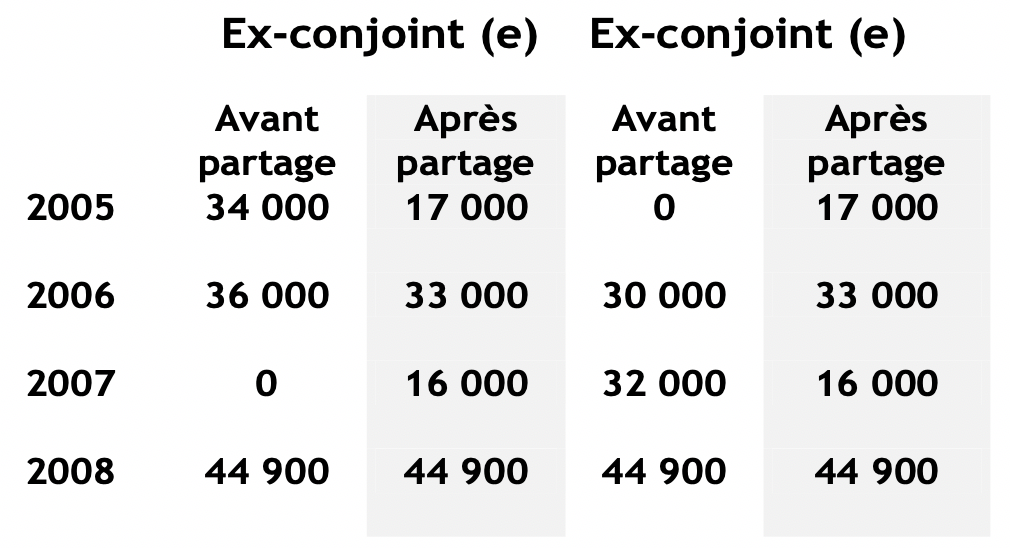
\includegraphics[scale=0.4]{src/ACT-1005/exemple-DIVORCE.png}
\end{center}


\subsubsection*{Division de la rente de retraite}
Conditions:
\begin{itemize}[leftmargin = *]
	\item	Les 2 conjoints doivent avoir au moins 60 ans;
	\item	\hl{L'objectif est l'égalité économique des conjoints};
	\item	La raison principale est fiscale et elle existe depuis 1994;
	\item	Si les conjoints sont mariés, c'est automatique à la demande d'un des deux sinon les deux doivent faire la demande.
\end{itemize}
\textcolor{red}{selon Isabelle, on ne va pas loin sur ce sujet.}


%%%	---------------
%%%	NOTE:
%%%	+	Je ne savais pas trop comment / si je devrais reformuler ces deux prochaines sous-sous-sections parce-que je n'ai pas écris grand chose à propos (AJVR).
%%%	---------------
\subsubsection*{Suffisance de la rente}
La PSV et le RRQ fournissent 40\% du salaire (MGA) et l'objectif est d'environ 70\%. Cela est atteint avec des RCR, le nouveau régime supplémentaire, etc.

\subsubsection*{Provisionnement}
Mélange entre un régime par répartition et un régime à capitalisation

\columnbreak

\subsection*{Régime supplémentaire}
\begin{rappel_enhanced}[Historique]
Entrée en vigueur:
\begin{description}
	\item[Premier volet]	1er janvier 2019 (régime S1);
	\item[Deuxième volet]	1er janvier 2024	(régime S2).
\end{description}
\end{rappel_enhanced}

\begin{conceptgen}{But}
\begin{itemize}[leftmargin = *]
	\item	Améliorer la qualité de vie des futurs retraités au Québec;
	\item	Assurer \hl{l'équité intergénérationnelle};
	\item	Harmoniser le RRQ avec le RPC;
	\item	Renforcer le financement du régime.
\end{itemize}
\end{conceptgen}

\begin{conceptgen}{Financement}
Le régime est \hl{obligatoire} et est en surplus du régime de base.

\begin{description}
	\item[S1]	Pourcentage applicable aux gains entre l'exemption générale et le MGA;
		\begin{itemize}[leftmargin = *]
		\item	La cotisation est équitablement séparée entre l'employeur et l'employé;
		\item	Va augmenter de 0.3\% en 2019 jusqu'à 2\% en 2023.
		\end{itemize}
	\item[S2]	Pourcentage applicable aux gains entre le MGA et le \textbf{MSGA};
		\begin{itemize}[leftmargin = *]
		\item	Le taux est de 8\% (4\% employeur et 4\% employé).
		\end{itemize}
	\item[MSGA]	Le nouveau maximum établit avec le régime supplémentaire.
		\begin{itemize}[leftmargin = *]
		\item	2024 MSGA = $1.07 \times$ MGA;
		\item	2025 MSGA = $1.14 \times$ MGA.
		\end{itemize}
	\item[Fiscalité]		Les cotisations sont déductibles d'impôts.
\end{description}
\end{conceptgen}

\begin{conceptgen}{Prestations}
Toute personne admissible au régime de base est automatiquement admissible au régime supplémentaire. Cependant, le montant de prestation est \hl{proportionnel} au nombre d'années de cotisation.\\

\paragraph*{Taux de remplacement de revenu}
\begin{description}
	\item[S1]	8.33\% de la moyenne des 40 gains admissibles les plus élevés;
	\item[S2]	33.33\% de la moyenne des 40 gains admissibles les plus élevés.
\end{description}


\paragraph*{Proportionnalité}
\begin{itemize}[leftmargin = *]
	\item	Chaque année de participation permet d'accumuler $1/40^{\text{ème}}$ du taux de remplacement de revenu;
	\item	Après 40 ans, ça permet de sélectionner les années ayant les salaires les plus élevés.
\end{itemize}

Les autres caractéristiques du régime (indexation, partage des droits, etc.) sont comme le régime de base.
\end{conceptgen}

\begin{conceptgen}{Provisionnement}
\begin{itemize}[leftmargin = *]
	\item	Régime capitalisé---les cotisations d'aujourd'hui serviront à payer les prestations de ces mêmes personnes;
	\item	Il y a donc beaucoup plus d'actifs et les revenus de placements vont représenter la majorité des revenus à long terme;
	\item	Les résultats du régime sont donc plus sensibles au taux de rendement des placements que le régime de base.
\end{itemize}
\end{conceptgen}

\columnbreak

\subsection*{L'invalidité}

\begin{definitionNOHFILL}[Invalide]
\begin{itemize}[leftmargin = *]
	\item	Incapacité grave et permanente;
	\item	Aucune amélioration possible;
	\item	Aucun emploi possible;
	\item	Durée indéterminée.
\end{itemize}

Cette définition est très différente que celle d'une compagnie d'assurance. \\
Par exemple, celle de SSQ:
\begin{center}
	\colorbox{asparagus}{\parbox{0.9\textwidth}{Limitation physique ou mentale, d’une durée temporaire ou permanente, qui empêche un assuré de remplir partiellement ou totalement les principales fonctions de son emploi.}}
\end{center}
\end{definitionNOHFILL}
		
\paragraph*{Note}	Les deux rentes sont payables mensuellement, indexées et imposables.
	
\subsubsection*{Rente d'invalidité}

\begin{conceptgen}{Admissibilité}
\begin{itemize}[leftmargin = *]
	\item	Être déclaré invalide \textit{par la Régie};
		\begin{itemize}[leftmargin = *]
		\item	Évaluation par l'équipe médicale de Retraite Québec.
		\end{itemize}
	\item	Avoir moins de 65 ans;
	\item	Avoir cotisé au moins 2 des 3 dernières années\\
			\textbf{ou}	\\
			5 des 10 dernières années	\\
			\textbf{ou}	\\
			la moitié des toutes les années dans la période cotisable (période d'au moins 4 ans)
\end{itemize}
\end{conceptgen}

\begin{definitionNOHFILL}[Délai de carence]
Période entre le moment où survient l'invalidité et le début des prestations.
\end{definitionNOHFILL}

%%%	----------------------------
%%%	NOTE
%%%	+	manque l'info sur le montant de prestation pour la rente d'invalidité.
%%%	----------------------------

\begin{conceptgen}{Prestation}
\begin{itemize}[leftmargin = *]
	\item	Le paiement est \hl{non-rétroactif} et payable à compter du \hl{quatrième mois suivant celui où le cotisant est reconnu invalide};
	\item	Le paiement cesse lorsqu'il y a :
		\begin{itemize}[leftmargin = *]
		\item	Décès (35\% des cas);
		\item	Cessation d'invalidité (2\% des cas);
		\item	L'obtention de l'âge de 65 ans dans quel cas elle est remplacée par une rente de retraite (63\% des cas).
		\end{itemize}
\end{itemize}
\end{conceptgen}

\subsubsection*{Rente d'enfant de personnes invalides}

\begin{conceptgen}{Admissibilité}
\begin{itemize}[leftmargin = *]
	\item	Cotisant admissible à une rente d'invalidité (RI);
	\item	Enfant du cotisant âgé de moins de 18 ans.
\end{itemize}
\end{conceptgen}

\begin{conceptgen}{Prestation}
\begin{itemize}[leftmargin = *]
	\item	En 2020, paiement mensuel fixe de 79.46\$;
	\item	Le paiement cesse lorsqu'il y a :
		\begin{itemize}[leftmargin = *]
		\item	L'obtention de l'âge de 18 ans par l'enfant;
		\item	Décès de l'enfant;
		\item	Cessation du paiement au cotisant.
		\end{itemize}
\end{itemize}
\end{conceptgen}

\columnbreak

\subsection*{Les prestations de survivants}

\begin{conceptgen}{Admissibilité}
Payable si la personne a décédée a cotisée:
\begin{itemize}[leftmargin = *]
	\item	1/3 des années de sa période cotisable (période d'au moins 3 années)	\\
%%%	--------------------------------
%%%	NOTE
%%%	+	Clarifier ici si c'est 3 ans ou 9 ans période cotisable ?
%%%	--------------------------------
			\textbf{ou}	\\
			10 années.
\end{itemize}
\end{conceptgen}

\subsubsection*{Rente de conjoint survivant}

\begin{definitionNOHFILL}[Conjoint]
\begin{itemize}[leftmargin = *]
	\item	Marriage	\\
			\textbf{ou}\\
			Union civile;
	\item	Conjoint de fait: 3 ans de vie commune (ou 1 s'il y a un enfant);
	\item	Inclut les couples du même sexe.
\end{itemize}
\end{definitionNOHFILL}

\begin{conceptgen}{Prestation}
\begin{itemize}[leftmargin = *]
	\item	Dans le cas d'un remariage, la rente continue d'être versée. \\
			S'il y a décès du nouveau conjoint, la rente la plus avantageuse des deux est versée;
	\item	Les prestations sont mensuelles.
\end{itemize}

Il y a plusieurs composantes à la rente donc certaines qui sont variables (c'est la seule rente avec cette caractéristique).
\begin{itemize}[leftmargin = *]
	\item	La partie uniforme varie selon l'âge et le nombre d'enfants à charge;
	\item	Il est possible que la rente soit réduite si la personne reçoit d'autres rentes (retraite, invalidité) mais est cumulative jusqu'à un maximum établi par la loi.
\end{itemize}
\begin{center}
	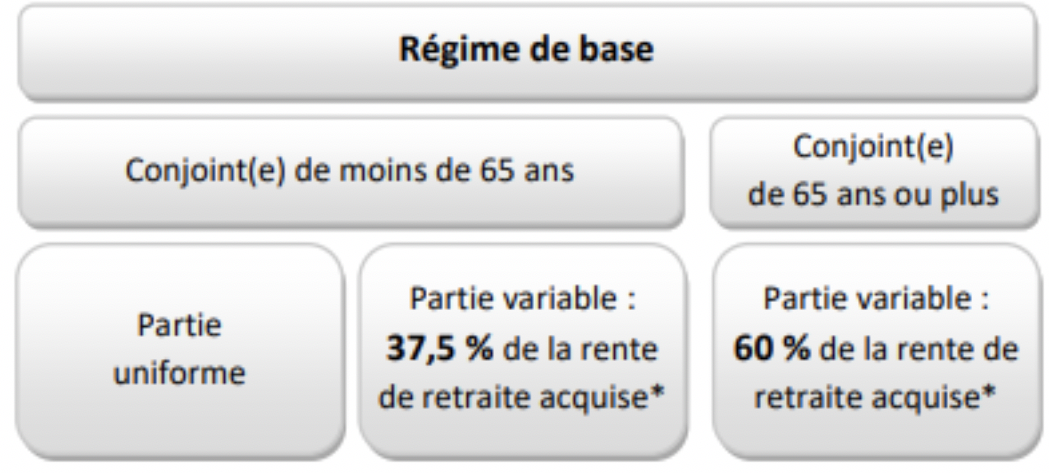
\includegraphics[scale=0.2]{src/ACT-1005/rente-conj-surv.png}
	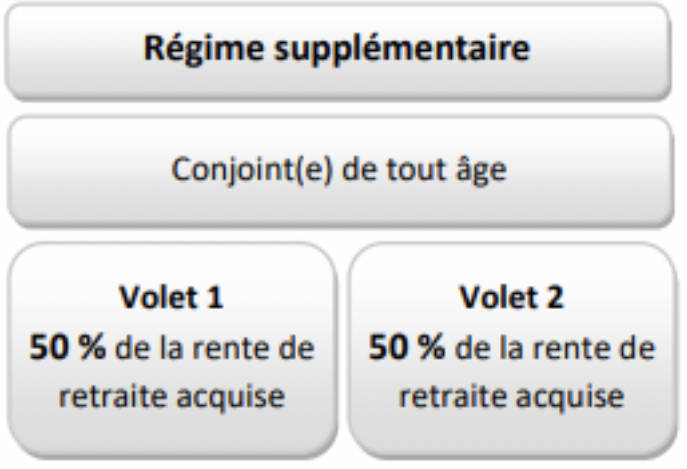
\includegraphics[scale=0.2]{src/ACT-1005/rente-conj-surv-2.png}
\end{center}
\end{conceptgen}

\subsubsection*{Rente d'orphelin}

\begin{conceptgen}{Détails}
\begin{itemize}[leftmargin = *]
	\item	Cesse à 18 ans (ou plus tard s'il est un étudiant à temps plein);
	\item	Montant mensuel fixe \red{(255.03\$ en 2020)};
	\item	Payable une seule fois même si les 2 parents décèdent.
\end{itemize}
\end{conceptgen}

\subsubsection*{Prestation de décès}

\begin{conceptgen}{Détails}
\begin{itemize}[leftmargin = *]
	\item	Montant unique de 2 500\$;
	\item	Priorité à la personne ayant acquitté les frais funéraires.
\end{itemize}
\end{conceptgen}

\newpage

\section{Les régimes volontaires d'épargne retraite (RVER)}

\subsection*{Objectifs}

\subsection*{Obligation d'offrir l'accès à un RVER}


\subsection*{Admissibilité}

\subsection*{Cotisations}

\subsection*{Placements}

\subsection*{Administration}

\subsection*{Fiscalité}

\subsection*{Pistes de réflexion}

\subsection*{Conclusion}

\subsection*{Exemple}

\newpage

\section{Les régimes complémentaires de retraite (RCR)}

\begin{definitionNOHFILL}[Définition du RCR]
Les compagnies peuvent mettre en place et offrir à leurs employés un régime de retraite qui vient en complément des régimes offerts par l'état. 
%%%	------------------------
%%%	NOTE
%%%	+	Mettre la définition? Je trouvais ça pourrait être trops lourd et j'étais un peu paresseux. (AJVR)
%%%	------------------------

\paragraph{Notes}
\begin{itemize}[leftmargin = *]
	\item	Traditionnellement, ce sont surtout des employés gouvernementaux et de grandes compagnies privées qui ont accès à des RCR; ils sont rares pour les employés de petites entreprises.
	\item	Le gouvernement accorde des avantages fiscaux pour encourager la mise en place de RCR.
	\item	Le fonctionnement est d'accumuler du rendements sur les cotisations pour payer les prestations à la retraite.
\end{itemize}
\end{definitionNOHFILL}

%%%	------------------------
%%%	NOTE
%%%	+	À faire (AJVR)
%%%	------------------------
\subsection*{Pour ou contre?}

Point de vue des:
\begin{description}
	\item[Gouvernements]	Les gouvernements les encouragent.
		\begin{itemize}[leftmargin = *]
		\item	Le RCR est un régime \textbf{agréé} car il est \textit{agréé} par la loi pour profiter d'avantages fiscaux;
		\item[$\color{blue}+$]	Utilité sociale des régimes de retraite;
		\item[$\color{blue}+$]	Réduction de la pauvreté parmi les aînés;
		\item[$\color{blue}+$]	Réduction du fardeau de la loi sur la sécurité du revenu;
		\item[$\color{blue}+$]	Accroissement du capital disponible pour investissement dans l'économie;
		\item[$\color{red}-$]	Diminution des revenus fiscaux.
		\end{itemize}
	\item[Entreprises]	L'employeur décide si il établit un RCR ou non, ainsi que ses modalités et prestations.
		\begin{itemize}[leftmargin = *]
		\item[$\color{blue}+$]	Recrutement et rétention des employés;
		\item[$\color{blue}+$]	Pression aux compétiteurs;
		\item[$\color{blue}+$]	Négociation syndicale;
%%%		--------------------
%%%		NOTE
%%%		+	Vérifier ce que ça veut dire efficacité fiscale. (AJVR)
%%%		--------------------
		\item[$\color{blue}+$]	\textit{Efficacité fiscale};
		\item[$\color{blue}+$]	Planification de la retraite des employés simplifiée.
		\item[$\color{red}-$]	Argent non disponible à d'autres fins (e.g., faire grossir la compagnie);
		\item[$\color{red}-$]	Complexité administrative.
		\end{itemize}
	\item[Employés]	L'employé bénéficie d'un RCR.
		\begin{itemize}[leftmargin = *]
		\item[$\color{blue}+$]	Meilleur revenu de retraite;
%%%		--------------------
%%%		NOTE
%%%		+	Vérifier ce que ça veut dire que les sommes sont provisionnées. (AJVR)
%%%		--------------------
		\item[$\color{blue}+$]	\textit{Sécurité des prestations---les sommes sont provisionnées};
		\item[$\color{blue}+$]	Planification de la retraite simplifiée;
		\item[$\color{blue}+$]	Contribution de l'employeur à l'épargne-retraite;
		\item[$\color{red}-$]	Préférence pour un salaire plus élevé plutôt que des prestations de retraite futures.
		\end{itemize}
\end{description}

\subsection*{Mise en place}
Il n'y a \hl{aucune obligation légale de mettre en place} un régime, \hl{n'y de couvrir tous les employés}. Cependant, on doit couvrir tous les employés d'une catégorie. Par exemple, on ne peut pas couvrir seulement 3 sur 4 des professeurs d'un département.

\paragraph*{Caractéristiques}	Les dispositions du régime sont déterminées par les compagnies.
\begin{description}
	\item[Participation]	Le régime peut être obligatoire ou facultatif;
		\begin{itemize}[leftmargin = *]
		\item	S'il est facultatif, on a le droit d'y participer plus tard.
		\end{itemize}
	\item[Admissibilité]	Le maximum de temps avant d'être admissible ne peut pas être plus que 2 ans;
	\item[Autres]	La compagnie décide comment gérer:
		\begin{itemize}[leftmargin = *]
		\item	Prestations en cas de décès, cessation d'emploi, d'invalidité;
		\item	La formule de calcul des cotisations;
		\item	L'âge de retraite;
		\item	Le service pris en considération;
		\item	Protection contre l'inflation.
		\end{itemize}
\end{description}


\subsection*{Contributions}
Les régimes peuvent être:
\begin{description}
	\item[contributifs]	cotisations d'employeurs \textit{et} d'employés.
	\item[non-contributifs]	cotisations seulement des employeurs.
\end{description}

\subsection*{Types de régimes}

\begin{description}
	\item[prestations déterminées]	On sait ce qu'on veut payer à la retraite.
	\item[cotisations déterminées]	On sait ce qu'on est prêt à payer sur le marché du travail.
	\item[hybrides]
\end{description}

\begin{center}
	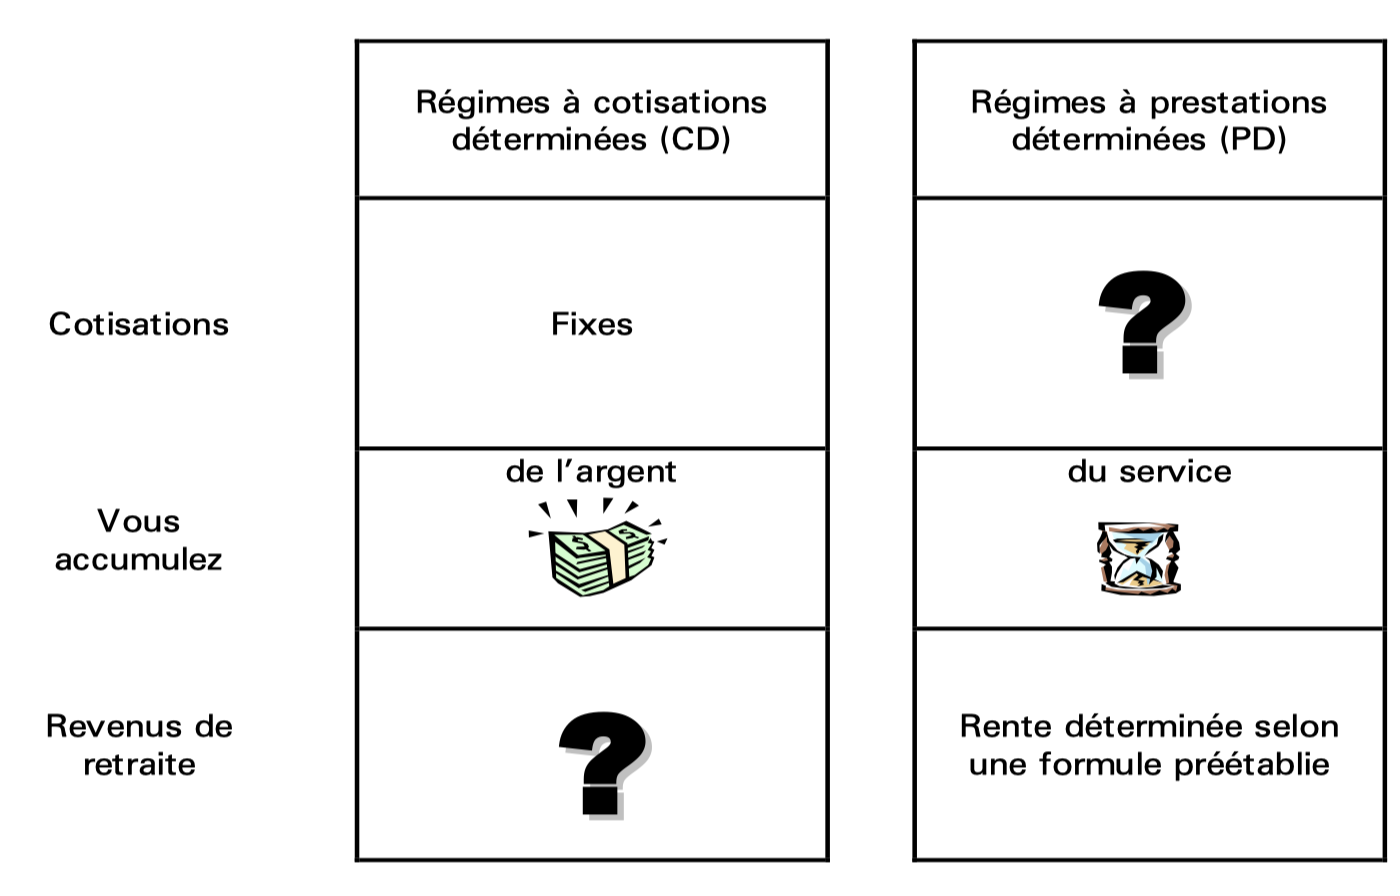
\includegraphics[scale=0.33]{src/ACT-1005/CD-PD-table.png}
\end{center}

\columnbreak

\section*{Régimes à prestations déterminées (PD)}

\begin{definitionNOHFILL}[Description]
Promesse (pas nécessairement garantie) de payer aux participants un montant de rente déterminé.

\paragraph{Notes}
\begin{itemize}[leftmargin = *]
	\item	Le \textit{niveau} des prestations est connu.\\
			C'est-à-dire que la \textit{formule} utilisée pour déterminer les prestations est connue mais \textbf{pas} le \textit{montant} comme tel;
	\item	Le montant varie habituellement selon le nombre d'années de service;
\end{itemize}
\begin{description}
	\item[Années de service]	Période calculée comme le nombre d'années de travail pour un même employeur.
\end{description}
\end{definitionNOHFILL}

\subsection*{Financement et investissement}

Le régime est financé par l'employeur (cotisations \textit{patronales}) et, si le régime est contributif, l'employé (cotisations \textit{salariales}).\\

Il n'y a aucune décision d'investissement pour le participant---l'\hl{employeur} investit les cotisations et \hl{est tenu au risque d'investissement}. \\

Il doit être en mesure de payer les prestations futures aux participants du régime et détermine les cotisations patronales en fonction d'une \textbf{évaluation actuarielle} périodique. 

\paragraph*{Note}	Les RCR sont exigés par la loi d'être par capitalisation afin d'assurer la sécurité des prestations promises.

\begin{definitionNOHFILLsub}[Évaluation actuarielle]
Détermine les cotisations (patronales et salariales s'il y a lieu) requises pour payer les prestations promises selon des \textit{hypothèses prévisionnelles}.

\begin{itemize}[leftmargin = *]
	\item	Exemples d'hypothèses prévisionnelles:
		\begin{itemize}[leftmargin = *]
		\item	Niveau futur des salaires.
		\item	Rendement des placements.
		\item	Moment du départ à la retraite.
		\item	Moment de décès.
		\end{itemize}
	\item	La loi requiert des évaluations aux 3 ans;
	\item	Les objectifs d'une évaluation sont:
		\begin{enumerate}
		\item	Estimer la \textbf{situation financière du régime} à une date donnée;
		\item	Recommander le niveau requis de cotisations;
		\item	Se conformer aux exigences légales.
		\end{enumerate}
\end{itemize}
\end{definitionNOHFILLsub}

\begin{definitionNOHFILLsub}[Situation financière du régime]
Les hypothèses de l'évaluation précédente vont rarement correspondre à la réalité ce qui impact la situation financière.\\

Le régime peut avoir un:
\begin{description}
%%%	--------------------
%%%	NOTE (AJvR)
%%%	+	Faudrait trouver un terme plus simple que "expérience" je trouve ça pourrait throw off du monde d'utiliser un terme actuarielle lorsque je ne pense pas que c'est vraiment nécessaire.
%%%	+	J'ai écris ce qui a été observé, qu'est-ce t'en penses?
%%%	--------------------
	\item[Déficit]	Lorsque les choses vont moins bien que prévu et qu'on a une perte selon ce qui a été observé (\textit{l'expérience}).
	\item[Surplus]	Lorsque les choses vont mieux que prévu et qu'on a un gain selon ce qui a été observé (\textit{l'expérience}).
\end{description}

Exemples d'événements qui peuvent mener à un déficit:
\begin{itemize}[leftmargin = *]
	\item	Niveau futur des salaires---les salaires sont plus élevés que prévu.
	\item	Rendement des placements---les rendements sont moins élevés que prévu.
	\item	Moment de décès---l'espérance de vie augmente.
\end{itemize}


\paragraph{Note} S'il y a un déficit, l'employeur doit verser des prestations additionnelles pour combler l'écart. Par contre, l'excédent d'\hl{un surplus ne vas pas automatiquement à l'employeur} et peut avoir d'autres utilités.
\end{definitionNOHFILLsub}

\subsection*{Types de formule pour calculer les prestations de rentes}

\begin{definitionNOHFILL}[Prestation forfaitaire]
La rente annuelle est un montant fixe pour chacune des années de service.

Désavantages:
\begin{itemize}
	\item[$\color{red}-$]	Ne tient pas compte du salaire du participant;
	\item[$\color{red}-$]	Les prestations sont en dollars courants et perdent leur pouvoir d'achat s'ils ne sont pas indexés;
	\item[$\color{red}-$]	Pas de notion du remplacement de revenu.
\end{itemize}

Avantages:
\begin{itemize}
	\item[$\color{blue}+$]	Facile à comprendre;
	\item[$\color{blue}+$]	Administration simple.
\end{itemize}
\end{definitionNOHFILL}

\subsubsection*{Régime pourcentage salaire}
La rente est fonction d'un pourcentage de salaire, ou d'une moyenne de salaires, pour chacune des années de service.

Il y a plusieurs types de régimes fonction du pourcentage de salaire.

\begin{definitionNOHFILL}[Salaire de carrière]
La rente est un pourcentage du salaire pour chaque année de participation au régime. \\
La rente payable à la retraite est donc la somme des rentes créditées annuellement durant la carrière du participant.

Désavantages:
\begin{itemize}
	\item[$\color{red}-$]	Les rentes créditées en début de carrière sont un faible pourcentage du salaire final.\\
							Il s'ensuit que c'est moins avantageux s'il y a une progression salariale importante;
	\item[$\color{red}-$]	Puisque la rente n'est pas basée sur des dollars actualisés, le taux de remplacement de revenu peut être faible;
	\item	La revalorisation périodique des rentes créditées serait nécessaire pour atténuer ce problème, mais c'est plus compliqué.
\end{itemize}

Avantages:
\begin{itemize}
	\item[$\color{blue}+$]	Simple à comprendre pour le participant;
	\item[$\color{blue}+$]	Simple à administrer et calculer.
\end{itemize}
\end{definitionNOHFILL}

\begin{conceptgen}{Exemple salaire de carrière}
Formule de rente: 2\% du salaire par année.\\
Adhésion le 1er janvier 2004 et retraite le 1er janvier 2007.
\begin{center}
\begin{tabular}{|	>{\columncolor{airforceblue}}c	| >{\columncolor{beaublue}}c | >{\columncolor{beaublue}}c  |}
\hline\rowcolor{airforceblue} 
\textcolor{white}{\textbf{Année}}	&	\textcolor{white}{\textbf{Salaire}}	&	\textcolor{white}{\textbf{Rente constituée}}		\\\specialrule{0.1em}{0em}{0.0em} 
2004	&	35 000\$	&	700\$	\\
2005&	40 000\$	&	800\$	\\
2006	&	33 000\$	&	860\$	\\\hline
\textbf{Total}	&		&	2 360\$	\\\hline
\end{tabular}
\end{center}
La rente annuelle payable par le régime est 2 360\$.
\end{conceptgen}

\begin{definitionNOHFILL}[Derniers salaires]
La rente est basée sur le nombre d'années de service \textit{et} sur le salaire moyen au cours des $Y$ années précédant la retraite.
\begin{itemize}[leftmargin = *]
	\item	Habituellement 3 ou 5 dernières années;
	\item	Ce sont les prestations les plus généreuses et coûteuses.
\end{itemize}

Désavantages:
\begin{itemize}
	\item[$\color{red}-$]	Administration plus complexe;
	\item[$\color{red}-$]	Coût du régime plus difficile à prévoir;
	\item[$\color{red}-$]	Pénalise les retraites progressives ou changements d'emploi en fin de carrière pour un salaire inférieur (si ce n'est pas prévu au régime).
\end{itemize}

Avantages:
\begin{itemize}
	\item[$\color{blue}+$]	Rente de retraite souvent liée aux meilleurs salaires;
	\item[$\color{blue}+$]	Puisque les augmentations salariales reflètent l'inflation, les rentes aussi.
\end{itemize}

\tcbline

\begin{center}
	\textbf{Salaire meilleurs années}
\end{center}
La rente est la moyenne des $Y$ années de meilleurs salaires. 

\begin{itemize}
	\item	Variante du régime meilleurs salaires;
	\item	L'avantage additionnel est la correction de l'impact négatif pour les personnes dont le salaire diminue à l'approche de la retraite.
\end{itemize}
\end{definitionNOHFILL}

\begin{conceptgen}{Exemple derniers et meilleurs salaires}
Formule de rente: 2\% $\times$ salaire final moyen sur 3 ans (SFM3) $\times$ années de participation (AP).\\
Adhésion le 1er janvier 1975 et retraite le 1er janvier 2010 (35 ans de service).
\begin{center}
\begin{tabular}{|	>{\columncolor{airforceblue}}c	| >{\columncolor{beaublue}}c |}
\hline\rowcolor{airforceblue} 
\textcolor{white}{\textbf{Année}}	&	\textcolor{white}{\textbf{Salaire}}	\\\specialrule{0.1em}{0em}{0.0em} 
1975		&	21 000\$		\\
\dots	&	\dots		\\
2006		&	70 000\$		\\
2007		&	74 000\$		\\
2008		&	77 000\$		\\
2009		&	65 000\$		\\\hline
\end{tabular}
\end{center}
\textbf{Selon derniers salaires}:
\begin{itemize}
	\item	SFM3 = $\frac{65000\$ + 77 000\$ + 74 000\$}{3} = 72 000\$$.
	\item	Rente annuelle de retraite = $2\% \times 72 000\$ \times 35 \text{ ans} = 50 400\$$.
\end{itemize}

\textbf{Selon meilleurs salaires}:
\begin{itemize}
	\item	SFM3 = $\frac{70 000\$ + 77 000\$ + 74 000\$}{3} = 73 667\$$.
	\item	Rente annuelle de retraite = $2\% \times 73 667\$ \times 35 \text{ ans} = 51 567\$$.
\end{itemize}
\end{conceptgen}

\begin{definitionNOHFILL}[Régimes flexibles]
Permets aux participants de verser des cotisations optionnelles (CO) pour acheter des prestations accessoires (PA) de leur choix.\\

Quelques exemples:
\begin{itemize}[leftmargin = *]
	\item	Bénéfice de décès avant retraite;
	\item	Indexation après la retraite;
	\item	Retraite anticipée sans réduction.
\end{itemize}

Notes
\begin{itemize}[leftmargin = *]
	\item	Les CO sont déductibles d'impôts et ne réduisent pas la marge permise au REER;
	\item[$\color{red}-$]	Administration plus compliquée;
	\item[$\color{blue}+$]	Flexible selon la situation de l'employé.
\end{itemize}
\end{definitionNOHFILL}

\columnbreak

\section*{Régimes à cotisations déterminées (CD)}

\begin{definitionNOHFILL}[Description]
Les cotisations (de l'employeur et l'employé) \textit{ou} la méthode utilisée pour les calculer sont déterminées à l'avance.

\paragraph{Notes}
\begin{itemize}[leftmargin = *]
	\item	Comme un compte de banque, la rente est fonction des cotisations;
	\item	Puisque le montant dépend de la valeur accumulée des cotisations, le moment de la retraite peut être problématique s'il y a une chute des marchés.
\end{itemize}
\end{definitionNOHFILL}


\subsection*{Investissement}

L'\hl{employé} \hl{assume le risque d'investissement} puisque son revenu à la retraite est directement lié au rendement du compte ayant les cotisations. \\

Il s'ensuit 	qu'il est généralement responsable du choix de placement et qu'il peut le changer en tout temps.

Puisque le but d'un régime à cotisations déterminées n'est pas de payer une rente de retraite, l'employé devra transférer le montant accumulé dans son compte.

\begin{definitionNOHFILLsub}[Formes de versement d'une rente]
Ce montant peut être transféré dans un:
\begin{description}
	\item[Compte de retraite immobilisé (CRI)]	L'équivalent d'un REER auquel on peut transférer des fonds provenant d'un RCR sauf qu'ils sont immobilisés.
		\begin{itemize}[leftmargin = *]
		\item	Le compte sert donc uniquement à accumuler de l'épargne-retraite.
		\item	Pour en tirer un revenu, l'individu doit soit transférer les sommes à un FRV ou acheter une rente viagère d'un assureur.
		\end{itemize}
	\item[Fonds de revenu viager (FRV)]	Fonds enregistré de revenu de retraite (FERR).
		\begin{itemize}[leftmargin = *]
		\item	Le fonds a une \textbf{limite} du montant pouvant être retiré annuellement.
		\item	Les sommes proviennent soit d'un CRI ou directement d'un RCR.
		\end{itemize}
	\item[Une rente]d'un assureur variant selon:
		\begin{itemize}[leftmargin = *]
		\item	le montant accumulé;
		\item	le taux d'intérêt de l'assureur (au moment du transfert);
		\item	l'âge du rentier (et co-rentier s'il y a lieu);
		\item	la forme (viagère ou différée) et les garanties de la rente.
		\end{itemize}
\end{description}
\end{definitionNOHFILLsub}

\paragraph{Note}	Les régimes à CD ont le danger que le cotisant n'ait pas assez de revenus à la retraite. Ceci peut être dû à un faible taux de cotisation salariale, un rendement faible du fonds de placement par défaut, etc.

\subsection*{Types de formule pour calculer les prestations de rentes}

\begin{definitionNOHFILL}[Cotisation déterminées]
Les cotisations sont: 
\begin{itemize}[leftmargin = *]
	\item	un pourcentage fixe du salaire \\
			\textbf{ou}
	\item	un montant donnée par années de service\\
			\textbf{ou}
	\item	un montant donnée par heure travaillé
\end{itemize}
\end{definitionNOHFILL}

\begin{conceptgen}{Exemple cotisation déterminée}
\begin{description}
	\item[Salaire]	40 000\$
	\item[Service]	22 ans
\end{description}
\tcbline
Exemple 1: 
\begin{description}
	\item[Taux de cotisation de l'employeur]	3\% du salaire;
	\item[Cotisation de l'employeur]	= 40 000\$ $\times$ 3\% = 1 200\$.
\end{description}	 
	
\tcbline

Exemple 2: 
\begin{description}
	\item[Taux de cotisation de l'employeur]	= taux de l'employé = 4\% du salaire;
	\item[Cotisation de l'employeur]	= 40 000\$ $\times$ 4\% = 1 600\$;
	\item[$\color{blue}+$]	Lorsque l'employeur cotise de façon égale à l'employé cela incite l'épargne.
\end{description}
	
\tcbline

Exemple 3: taux de cotisation de l'employeur selon une table:
\begin{center}
\begin{tabular}{|	>{\columncolor{white}}c	| >{\columncolor{white}}c |}
\hline\rowcolor{airforceblue} 
\textcolor{white}{\textbf{Années de service $x$}}	&	\textcolor{white}{\textbf{Rapporté}}	\\\specialrule{0.1em}{0em}{0.0em} 
$x \le$ 10 ans	&	75\%	\\
10 ans $< x <$ 20 ans	&	100\%	\\
$x \ge$ 20 ans	&	125\%	\\\hline
\end{tabular}
\end{center}
\begin{description}
	\item[Taux de cotisation de l'employeur]	= taux de l'employé $\times$ 1.25 = 4\% $\times$ 1.25 = 5\% du salaire;
	\item[Cotisation de l'employeur]	= 40 000\$ $\times$ 5\% = 2 000\$;
	\item[$\color{blue}+$]	Reconnait le service,
\end{description} 
\end{conceptgen}

\begin{definitionNOHFILL}[Avec participation aux bénéfices]
Les cotisations de l'employeur sont liées à la rentabilité de l'entreprise.

\begin{itemize}[leftmargin = *]
	\item	L'agence du revenu du Canada (ARC) exige que l'entreprise verse un minimum de 1\% de la masse salariale.
	\item	La répartition se fait selon une formule basée sur les années de service et/ou le salaire.
\end{itemize}

Désavantages:
\begin{itemize}
	\item[$\color{red}-$]	Augmente l'incertitude liée au montant de rente;
\end{itemize}

Avantages:
\begin{itemize}
	\item[$\color{blue}+$]	Peut motiver les employés à être plus productifs.
\end{itemize}
\end{definitionNOHFILL}

\begin{definitionNOHFILL}[Régime simplifié]
Régime à CD administré par un établissement financier offert aux employeurs (mélange de CD et REER).

\begin{itemize}[leftmargin = *]
	\item	Ce régime est un mélange de fonds immobilisés et non immobilisés. \\
			Les cotisations de l'employeur et de l'employé (à moins d’avis contraire de l’employeur) sont immobilisées. \\
			Les cotisations additionnelles de l'employé sont non immobilisées.
\end{itemize}
\end{definitionNOHFILL}

\newpage

\section*{Hybrides}

\begin{definitionNOHFILL}[Description]
Régime à cotisations \textbf{et} prestations déterminées; les cotisations ainsi que la méthode du calcul de la rente sont prédéterminées.
\end{definitionNOHFILL}

\subsection*{Types de formule pour calculer les prestations de rentes}

\begin{definitionNOHFILL}[Cotisations et prestations déterminées]
Verse le maximum entre la \textcolor{teal}{rente à PD} et \textcolor{teal}{la rente pouvant être souscrite des cotisations accumulées}.


Désavantages:
\begin{itemize}
	\item[$\color{red}-$]	Plus d'administration par l'employeur qui doit gérer les investissements.
\end{itemize}

Avantages:
\begin{itemize}
	\item[$\color{blue}+$]	Réduis l'incertitude d'un régime à CD, car il y garantit un revenu minimal à la retraite;
	\item[$\color{blue}+$]	Détermine si c'est un régime à PD ou CD seulement au moment de la retraite.
\end{itemize}
\end{definitionNOHFILL}

\begin{definitionNOHFILL}[Combiné]
Additionne les rentes de la composante à PD et de la composante à CD

\begin{itemize}[leftmargin = *]
	\item	Souvent l'employeur fournit la composante à PD et l'employé la composante à CD.
\end{itemize}

Désavantages:
\begin{itemize}
	\item[$\color{red}-$]	Complexe à administrer et expliquer.
\end{itemize}
\end{definitionNOHFILL}

\columnbreak

\section*{Autres caractéristiques}

\subsection*{Coordination avec les régimes d'État}

\subsection*{Enregistrement et fiscalité}

Ce que régit:
\begin{description}
	\item[Loi du RCR du Québec]
	\item[Loi de l'impôt sur le revenu (LIR)]
\end{description}

Réforme de 1991 de la LIR

\subsection*{Âge d'admissibilité à la retraite}
\begin{itemize}[leftmargin = *]
	\item	
\end{itemize}

\subsection*{Prestations de décès avant la retraite}
\begin{itemize}[leftmargin = *]
	\item	Obligatoire pour le régime de définir les prestations qui le conjoint, ou autres, recevront en cas de décès avant la retraite du participant.
	\item	Le montant de prestation doit être, au minimum, égal aux sommes versées accumulées du participant;
%%%	------------------------
%%%	NOTES
%%%	+	Quoi? (AJVR)
%%%	------------------------
	\item	\textit{immobilisé si le survivant est un conjoint}?
	\item	Normalement un seul paiement forfaitaire.
\end{itemize}

\subsection*{Prestations de décès pendant la retraite}
\begin{itemize}[leftmargin = *]
	\item	Loi prévoit le versement d'une rente de survivant au conjoint admissible du retraité;
	\item	C'est une \textbf{rente réversible};
	\item	Doit être d'au moins 60\% de la rente du retraité;
	\item	Versé même si le conjoint se remarie.
\end{itemize}

\subsection*{Protection contre l'inflation}
\begin{itemize}[leftmargin = *]
	\item	La loi n'oblige pas l'indexation post-retraite.
\end{itemize}

\newpage

\section*{Résumé des différents RCR}

\subsection*{Régimes à prestations déterminées (PD)}
\begin{center}
	\textbf{Employé}
\end{center}
Pour
\begin{itemize}
	\item[$\color{blue}+$]	Permets de comprendre la notion de remplacement de revenus.
	\item[$\color{blue}+$]	L'employeur assume le risque de placement.
	\item[$\color{blue}+$]	Bon pour les employés avec beaucoup d'années de service.
	\item[$\color{blue}+$]	Les cotisations salariales sont déductibles d'impôts.
	\item[$\color{blue}+$]	Les cotisations optionnelles (CO) permettent d'optimiser la valeur fiscale.
	\item[$\color{blue}+$]	Possibilité de racheter des années de service antérieures.
\end{itemize}

Contre
\begin{itemize}
	\item[$\color{red}-$]	Plus compliqué à comprendre.
	\item[$\color{red}-$]	Fonds immobilisés non disponibles pour autre chose.
	\item[$\color{red}-$]	Le facteur d'équivalence (FE) réduit les marges au REER.
\end{itemize}

\begin{center}
	\textbf{Employeur}
\end{center}
Pour
\begin{itemize}
%%%	---------------------
%%%	NOTE (AJvR)
%%%	+	Pas certain de bien saisir ce que ça veut dire:
%%%	---------------------
%	\item[$\color{blue}+$]	Développement des programmes de retraite pour gérer la fluctuation de la main-d'œuvre (retraite anticipée).
	\item[$\color{blue}+$]	Possibilité d'augmenter les prestations au besoin.
	\item[$\color{blue}+$]	Premier bénéficiaire des gains sur les rendements et l'expérience (surplus).
	\item[$\color{blue}+$]	Cotisations patronales déductibles d'impôts.
\end{itemize}

Contre
\begin{itemize}
	\item[$\color{red}-$]	Coût d'administration plus élevé.
	\item[$\color{red}-$]	Difficile de prévoir la charge de retraite et impossible de prévoir le coût réel du régime.
	\item[$\color{red}-$]	Plus de communication est nécessaire.
\end{itemize}

\subsection*{Régimes à cotisations déterminées (CD)}
\begin{center}
	\textbf{Employé}
\end{center}
Pour
\begin{itemize}
	\item[$\color{blue}+$]	Facile à comprendre.
	\item[$\color{blue}+$]	Flexibilité des placements.
\end{itemize}


Contre
\begin{itemize}
	\item[$\color{red}-$]	Employé assume le risque d'investissement avant \textbf{et} après sa retraite.
	\item[$\color{red}-$]	Le montant de prestation de retraite n'est pas prévisible.
\end{itemize}

\begin{center}
	\textbf{Employeur}
\end{center}
Pour
\begin{itemize}
	\item[$\color{blue}+$]	Tenue de dossiers simple.
	\item[$\color{blue}+$]	Coûts facilement budgétisés.
	\item[$\color{blue}+$]	Aucun risque d'investissement.
%%%	--------------------
%%%	NOTE (AJvR)
%%%	+	Pas sur de ce que ça veut dire exactement / pourquoi c'est une bonne chose?
%%%	+	Me semble la compagnie ne serait pas contente d'avoir des fonds immobilisés puisqu'elle ne peut pas faire un rendement d'investissement / l'utiliser pour expansion / etc.?
%%%	--------------------
%	\item[$\color{blue}+$]	L'argent sera utilisé pour la retraite (immobilisation)
\end{itemize}

Contre
\begin{itemize}
	\item[$\color{red}-$]	Administration des RCR réglementée.
%%%	--------------------
%%%	Voir note ci-dessus
%%%	--------------------
%	\item[$\color{red}-$]	Pas d'outils pour gérer les ressources humaines. 
%%%	--------------------
%%%	NOTE
%%%	+	Pourquoi c'est un négatif pour eux?
%%%	+	Ce ne serait pas uniquement un négatif pour les employés ou est-ce que je manque de quoi ici?
%%%	--------------------
	\item[$\color{red}-$]	Montant de prestation non-prévisible.
	\item[$\color{red}-$]	Certaine responsabilité sur les (mauvais) placements des employés et donc le besoin des informer sur le risque/rendement des placements.
	\item[$\color{red}-$]	Prestations peuvent être inadéquate pour les employés déjà âgés.
\end{itemize}

\subsection*{Régimes hybrides}
\begin{center}
	\textbf{Employé}
\end{center}
Pour
\begin{itemize}
	\item[$\color{blue}+$]	
\end{itemize}


Contre
\begin{itemize}
	\item[$\color{red}-$]	
\end{itemize}

\begin{center}
	\textbf{Employeur}
\end{center}
Pour
\begin{itemize}
	\item[$\color{blue}+$]	
\end{itemize}

Contre
\begin{itemize}
	\item[$\color{red}-$]	
\end{itemize}

\end{multicols*}
\end{document}
